
\documentclass{article}
\usepackage{graphicx} % Required for inserting images
\usepackage{fancyhdr} % Required for header and footer configuration
\usepackage[a4paper, margin=2.5cm, left=1.5cm, right=1.5cm, bottom=4cm]{geometry} % Required for setting page margins
\usepackage[T1]{fontenc}
\usepackage[default,oldstyle,scale=1]{opensans} % Utilizzo del font Open Sans
\usepackage{lipsum}
\usepackage{makeidx}
\usepackage{booktabs}
\usepackage{tabularray}
\usepackage[colorlinks=true, linkcolor=black, urlcolor=blue, citecolor=blue]{hyperref}
\usepackage{tabularx}
\usepackage{makecell}
\usepackage{enumitem} % Pacchetto per la personalizzazione degli elenchi
\usepackage{booktabs}
\usepackage{subcaption}
\usepackage{pgfplots}
\usepackage{float}
\usepgfplotslibrary{dateplot} % Per gestire gli assi con date
\usepackage{soul}

% Configure header and footer for the first page
\fancypagestyle{firstpage}{
    \fancyhf{} % Clear header and footer
    \renewcommand{\headrulewidth}{0pt} % Remove header rule line
    \lhead{} % Header on the left
    \chead{} % Header in the center
    \rhead{} % Header on the right
    \lfoot{} % Footer on the left
    \cfoot{\vspace{5pt}\\\hrulefill\\\vspace{10pt}\textbf{BeeLive}\\Gruppo 21} % Footer in the center
    \rfoot{\vspace{32.5pt}\\\thepage} % Footer on the right
}

% Configure header and footer for non-plain pages (second page onwards)
\fancypagestyle{nonplain}{
    \fancyhf{} % Clear header and footer
    \lhead{} % Header on the left
    \chead{} % Header in the center
    \rhead{
\includegraphics[width=2cm]{Images/BeeLive-Logo.png}\\\vspace{2pt}} % Header on the right
    \lfoot{} % Footer on the left
    \cfoot{\vspace{5pt}\\\hrulefill\\\vspace{10pt}\textbf{BeeLive}\\Gruppo 21} % Footer in the center
    \rfoot{\vspace{32.5pt}\\\thepage} % Footer on the right
}

% Adjust vertical space between header and text                                    
\setlength{\headsep}{65pt} 
% Adjust vertical space between text and footer
\setlength{\footskip}{0pt} 

\title{
\includegraphics[width=0.75\textwidth]{Images/BeeLive-Logo.png}\\\vspace{100pt}
\LARGE{\textbf{BeeLive\\Deliverable 4}}}
\author{Gruppo 21:\\
Cipriani Pietro, 226959\\
Orlando Dennis, 227688\\
Ziviani Elia, 228172}
\date{11 Giugno 2024}

\makeindex % Indica che vogliamo creare un indice

\begin{document}

\maketitle
\thispagestyle{firstpage} % Apply firstpage style to the first page
\clearpage

\pagestyle{nonplain} % Apply non-plain style to subsequent pages

\renewcommand{\contentsname}{Indice}
\tableofcontents

\clearpage

\section{Revisione}
\label{sec:revisione}
La struttura del progetto, paragonandola a quella riportata nel deliverable precedente, è rimasta pressoché invariata.\\
Le uniche modifiche che sono state apportate sono relative al product backlog (\ref{tab:product-backlog}).
Le modifiche di cui si parla sono:
\begin{itemize}
    \item Ridefinizione della user story \textbf{Visualizzazione dei dettagli del singolo evento}, in quanto nello scorso documento risultava poco chiara e di difficile comporensione.
    \item Aggiunta di una nuova user story, \textbf{Accesso al programma desktop}, in quanto ritenuta necessaria per la completezza del progetto.
\end{itemize}
Questa user story è stata aggiunta in quanto ritenuta necessaria per il corretto funzionamento del progetto.\\
Si tratta di permettere, all'utente autorizzato, di accedere all'applicativo desktop in modo da poter operare sulle criticità associate.\\

\clearpage

\section{Introduzione}

\subsection{Componenti del gruppo}
\begin{itemize}
    \item Cipriani Pietro, matricola 226959, \lbrack\href{https://github.com/pietrocipriani}{github profile}\rbrack
    \item Orlando Dennis, matricola 227688, \lbrack\href{https://github.com/dennisorlando}{github profile}\rbrack
    \item Ziviani Elia, matricola 228172, \lbrack\href{https://github.com/ELI20ZIVI}{github profile}\rbrack
\end{itemize}

\subsection{Scopo del progetto}

Lo scopo del progetto 'BeeLive' è quello di creare un sistema informativo, dedicato ai cittadini di Trento, che permetta di reperire facilmente le informazioni riguardanti gli eventi che influenzano la viabilità all'interno del Comune di Trento. Il risultato finale prevede un applicazione mobile che mostri visualmente le variazioni della viabilità in città, informando gli utenti di eventuali modifiche che potrebbero intaccarli direttamente. 

\subsection{Link utili}
Il seguente link consente l'accesso alla nostra repository github:
\href{https://github.com/ELI20ZIVI/BeeLive/}{Repository GitHub}\\
La repository è stata creata appena il corso è cominciato, infatti è risultata utile fin dall'inizio al fine di scrivere in modo collaborativo i primi deliverable.\\
E' stato deciso di integrare in questa repository anche le fasi di sprint in quanto come team riteniamo utile la possibilità di accedere alla documentazione redatta nei precedenti deliverable.\\\\
Il seguente è il link ad Apiary, strumento col quale abbiamo creato e documentato approfonditamente le API utilizzate nel progetto:
 \href{https://beelive.docs.apiary.io/#}{Link Apiary}\\\\
Per testare il progetto è sarà necessario installare i due applicativi (Mobile e Desktop). Il seguente è un link alla prima \textit{Github Release} che abbiamo creato e che include le applicazioni precompilate, scaricabili ed utilizzabili: \href{https://github.com/ELI20ZIVI/BeeLive/releases/tag/0.1}{Github Release 0.1}\\
L'account da utilizzare per il login all'applicativo desktop è il seguente:
\begin{itemize}
    \item Utente Autorizzato: Username: \textit{authz\_user}, Password: \textit{pesettodaunchilo}
\end{itemize}
\noindent
Il portale CasDoor dell'applicativo desktop permette di creare ulteriori utenti, però questi utenti non sono autorizzati ad effettuare modifiche o inserire eventi, in quanto tale autorizzazione è stata garantita, manualmente, solamente all'utente \textit{authz\_user}.
\\
Il login all'applicativo mobile è opzionale: attualmente, le funzionalità di un utente autenticato sono le stesse degli utenti non autenticati. 

\clearpage

\section{Sezione generale}

\subsection{Strategia di Branching}
Anche per questo secondo sprint è stata evitata la strategia di branching "Master only": come descritto nel documento "Deliverable 3". La creazione e l'utilizzo di un unico branch principale \textit{main} avrebbe causato problemi di collaborazione e conflitti nel momento in cui tutti i componenti sarebbero andati a lavorare conteporaneamente a stesse sezioni del progetto.\\\\
\noindent
Abbiamo deciso di mantenere la stessa metodologia di branching dello scorso sprint, ossia il \textit{GitFlow Workflow}. Una volta ritenute soddisfacenti le modifiche e le feature di una "feature branch", questa verrà integrata in \texttt{develop}.\\
La branch \texttt{main} è la branch stabile in cui vengono effettuate le pull requests da \texttt{develop} solo una volta testate, determinando il rilascio della \textit{release}.\\\\

\noindent
Tramite questo approccio siamo riusciti a minimizzare i problemi di  collaborazione tra i membri del team, riducendo i conflitti e le inconsistenze nel codice, facilitando così la gestione delle diverse attività in corso e mantenendo inoltre una mappatura di tutte le diverse modifiche e progressi del progetto. Così facendo è stata conservata la storia del codice in maniera ben strutturata.

\noindent
Verso la fine del precedente sprint, abbiamo unificato le diverse branches in \texttt{develop} e, all'inizio di questo sprint, abbiamo nuovamente effettuato dei rebranching da \texttt{develop} in modo da lavorare sulle singole features.
Lo storico della nostra strategia di branching e' visualizzabile sotto il tool "Network Graph" fornito da github, accessibile da questo link:
\href{https://github.com/ELI20ZIVI/BeeLive/network}{Network Graph}\\

\noindent
Segue una lista dei branch utilizzati per lo sviluppo del progetto; da notare che molte di queste branches sarebbero dovute essere eliminate a seguito del primo sprint ma, come suggerito dai docenti, le abbiamo tenute.

\subsubsection{\texttt{main}}

Il branch principale del progetto, in cui vengono integrate tutte le funzionalità completate e testate.\\
Tutte le funzionalità all'interno di questo branch sono considerate terminate e funzionanti, pronte per essere rilasciate.

\subsubsection{\texttt{develop}}

Il branch di sviluppo del progetto, in cui vengono integrate tutte le funzionalità completate e testate.\\
Non e' pensato propriamente come il branch in cui vengono rilasciate le funzionalita' ma piuttosto come un branch di supporto per il branch principale, infatti in questo branch vengono prima caricate le funzionalita' dagli altri branch specifici e successivamente testate.\\
Una volta che sono considerate funzionanti sono quindi integrate nel branch principale.

\subsubsection{\texttt{preview}}

Branch (obsoleto) dedicato allo sviluppo del mockup dell'interfaccia grafica dei due applicativi.\\
E' stato utilizzato al momento della prima presentazione del progetto per mostrare il lavoro svolto ai committenti e per ricevere feedback su eventuali modifiche da apportare.\\
Integra dei mockup delle varie interfacce, desktop e mobile, che andranno sviluppate.\\
Parte della preview relativa all'applicativo desktop è stata poi utilizzata in \texttt{da\_frontend} come punto di partenza per l'interfaccia.

\subsubsection{\texttt{deliverable}}

Branch dedicato alla stesura dei vari documenti di deliverable che è stato creato per mantenere separata la stesura della documentazione dal codice sorgente e per rispettare la metodologia di branching.

\subsubsection{\texttt{refactoring}}

Questo branch nasce per la necessità di effettuare refactoring sul codice prodotto. Prima di eseguire il merge in \texttt{main} spesso risulta necessario effettuare delle modifiche al codice per renderlo più leggibile, mantenibile e performante.\\
Avendo un ambiente separato si annulla la possibilità di introdurre errori nel codice principale.

\subsubsection{\texttt{deployment}}

Branch dedicato alla preparazione del deploy del progetto.\\
Vengono preparate tutte le componenti alla fase di deploy, come la creazione dei file di configurazione, la preparazione dei file per il deploy e la creazione di script per automatizzare il deploy.

\subsubsection{\texttt{management-server}}

Branch dedicato allo sviluppo del server di gestione, il server utilizzato dall'applicativo desktop (Quindi dagli utenti autorizzati) per eseguire tutte le operazioni di gestione degli eventi.

\subsubsection{\texttt{public\_server}}

Similmente al branch precedente, questo branch è dedicato allo sviluppo del server pubblico, il server utilizzato dall'applicativo mobile (Quindi dagli utenti comuni) per la visualizzazione degli eventi e le varie impostazioni dell'applicativo.

\subsubsection{\texttt{da\_frontend}}

Branch (feature) dedicato allo sviluppo dell'interfaccia grafica dell'applicativo desktop.\\
In questo branch vengono sviluppate tutte le componenti che caratterizzano l'interfaccia grafica dell'applicativo desktop.

\subsubsection{\texttt{da\_authn}}

Il branch (feature) è dedicato allo sviluppo del modulo di autenticazione dell'applicativo desktop.\\
Include infatti tutto il codice e la logica necessari all'autenticazione degli utenti autorizzati e dell'utente amministratore all'applicativo desktop.

\subsubsection{\texttt{da\_event\_list}}

Branch (feature) di sviluppo della funzionalità di visualizzazione a lista degli eventi a disposizione dell'utente che ha eseguito il login all'applicativo desktop.\\
E' integrata tutta la logica di richiesta delle informazioni al server e di visualizzazione delle stesse in modo chiaro e ordinato.

\subsubsection{\texttt{ma\_client}}

Branch (feature) dedicato allo sviluppo del client mobile, i.e. l'applicazione mobile utilizzata dagli utenti comuni (autenticati e non) che intendono visualizzazione le criticita' presenti in citta'.\\
Il branch, una volta concluso lo sviluppo dell'applicativo, e' stato integrato nel branch \texttt{develop} per i test in associata con tutti gli altri moduli.


\subsubsection{\texttt{ma\_screen}}

Branch (feature) dedicato alla creazione delle schermate dell'applicativo mobile, i.e. tutte le schermate che l'utente visualizzera' durante l'utilizzo dell'applicativo.\\
Questo branch è stato integrato in \texttt{ma\_client} in quanto sua dipendenza.

\subsubsection{\texttt{ma\_details}}

Il branch (feature) nasce con lo scopo di mantenere il codice dell'interfaccia di visualizzazione degli eventi e dei rispettivi sottoeventi sull'applicativo mobile.
Branch successivamente integrato in \texttt{ma\_client} in quanto sua dipendenza.

\subsubsection{\texttt{ma\_map}}

Branch (feature) utilizzato per sviluppare la libreria che permette di integrare la mappa interattiva all'interno dell'applicativo mobile.\\
Questa libreria permette di visualizzare in modo chiaro e intuitivo le criticita' presenti in citta' e di visualizzare la posizione degli eventi.

\subsubsection{\texttt{ws-fetch-event}}

Branch (feature) dedicato allo sviluppo del webserver pubblico, i.e. il webserver in cui sono stati implementati gli endpoint API dedicati al fetching di eventi ad opera dell'applicativo mobile.\\
Una volta che il modulo e' stato completato, e' stato integrato nel branch \texttt{develop} per i test con tutti gli altri moduli.

\subsubsection{\texttt{ws-insert-event}}

Branch (feature) dedicato allo sviluppo del webserver gestionale, i.e. il webserver in cui sono stati implementati gli endpoint API dedicati all'inserimento degli eventi all'interno del sistema ad opera dell'applicativo desktop. \\
Utile allo sviluppo del modulo utilizzato dall'applicativo desktop per l'inserimento delle criticita' in citta'.
Una volta che il modulo e' stato completato, e' stato integrato nel branch \texttt{develop} per i test con tutti gli altri moduli.\\
Delle versioni intermedie di questa branch sono state usate da altre branches, in particolare da \texttt{da\_desktop}, in quanto necessaria per effettuare il testing di quest'ultima.

\subsubsection{\texttt{hotfixes}}
È stato necessario effettuare correzioni alla branch \texttt{hotfixes} al fine di correggere bug e incongruenze.\\
L'utilizzo intensivo di questa branch è dovuto al fatto che, visto lo scope del progetto, non è stato possibile effettuare code reviews delle pull requests.

\subsubsection{\texttt{testing}}
I tests sono stati scritti su branch a parte. Sebbene molti degli integration tests siano relativi a specifiche features, non è stato possibile implementarli in contemporanea per questioni di tempo.

\clearpage

\subsection{Product Backlog}
\label{tab:product-backlog}
Nella pagina seguente vi è riportato il product backlog che abbiamo sviluppato per questo progetto. E' possibile notare una linea di demarcazione che limita inferiormente le entries selezionate per il primo sprint.

\begin{table}[!ht]
    \centering
    \renewcommand{\arraystretch}{1.3} % Imposta lo spazio verticale delle righe
    \begin{tabularx}{\textwidth}{| r | X | r | r |}
        \Xhline{2pt}
        \makecell{\textbf{Nome}} & \makecell{\textbf{User story}} & \makecell{\textbf{Priorità}} & \makecell{\textbf{Stima}} \\
        \Xhline{2pt}
        \makecell{Accesso alle\\criticità} & \makecell{Da utente, voglio essere in grado di visualizzare la lista\\degli eventi che ci sono in città} & \makecell{200} & \makecell{8}\\
        \hline
        \makecell{Accesso al\\programma\\desktop} & \makecell{Da utente autorizzato, voglio essere in grado di accedere\\all'applicativo desktop in modo da poter operare\\sulle criticità a me associate} & \makecell{190} & \makecell{8}\\
        \hline
        \makecell{Aggiunta eventi\\da utente\\autorizzato} & \makecell{Da utente autorizzato, devo essere in grado di aggiungere degli eventi\\in modo da comunicare la loro presenza agli utenti} & \makecell{180} & \makecell{8}\\
        \hline
        \makecell{Registrazione e\\accesso all'\\app mobile} & \makecell{Da utente, voglio essere in grado di poter registrare un account\\in modo da poter salvare le mie impostazioni\\e le aree di interesse che ho impostato} & \makecell{170} & \makecell{8}\\
        \hline
        \makecell{Visualizzazione\\criticità\\su mappa} & \makecell{Da utente, voglio visualizzare su una cartina le zone colpite dai diversi\\eventi, in modo da capire visivamente se in una zona che mi\\interessa vi è un evento attivo} & \makecell{160} & \makecell{6}\\
        \hline
        \makecell{Visualizzazione\\dei dettagli del\\singolo evento} & \makecell{Da utente, voglio avere la possibilità di accedere ad una\\visualizzazione e descrizione più dettagliata di un\\evento in modo da conoscerne meglio le specifiche} & \makecell{150} & \makecell{6}\\
        \hline
        \makecell{Modifica\\eventi} & \makecell{Da utente autorizzato, devo essere in grado di modificare degli eventi\\in modo da evitare errori comunicativi} & \makecell{75} & \makecell{2}\\
        \hline
        \makecell{Eliminazione\\eventi} & \makecell{Da utente autorizzato, devo essere in grado di eliminare degli eventi} & \makecell{40} & \makecell{2}\\
        \Xhline{2pt}
        \makecell{Impostazione\\categorie\\d'interesse\\per gli eventi} & \makecell{Da utente, voglio essere in grado di impostare le categorie di eventi\\alle quali io sono interessato, in modo che la lista di eventi visibile\\dall'applicazione contenga solamente gli eventi che mi interessano,\\e in modo che io non venga notificato di alcun evento\\che io non ritenga appartenere ad una categoria interessante} & \makecell{100} & \makecell{5}\\
        \hline
        \makecell{Impostazione\\zone\\d'interesse} & \makecell{Da utente, voglio essere in grado di impostare delle zone di interesse,\\in modo che io venga notificato di qualsiasi evento che insorga\\in una di queste zone} & \makecell{90} & \makecell{7}\\
        \hline
        \makecell{Visualizzazione\\eventi\\di competenza} & \makecell{Da utente autorizzato, devo essere in grado di visualizzare gli eventi\\di mia competenza, in modo da sapere quali eventi sono stati creati e\\monitorare il loro stato} & \makecell{80} & \makecell{5}\\
        \hline
        \makecell{Accesso\\account\\utente} & \makecell{Da utente registrato, voglio essere in grado di poter accedere al\\mio account in modo da poter riottenere le aree di interesse e\\le impostazioni che ho precedentemente salvato} & \makecell{70} & \makecell{3}\\
        \hline
        \makecell{Visualizzazione\\eventi\\di categorie\\di interesse} & \makecell{Da utente, voglio essere in grado di visualizzare solo\\eventi di categorie di interesse} & \makecell{60} & \makecell{3}\\
        \hline
        \makecell{Selezione\\percorso} & \makecell{Da utente, voglio essere in grado di selezionare un percorso a partire\\da dei waypoint, per impostare dei percorsi di interesse} & \makecell{40} & \makecell{2}\\
        \hline
    \end{tabularx}
    \caption{Product backlog}
\end{table}

\clearpage

\subsection{Definition of "Done"}
La seguente 'Definition of Done' è basata su una valutazione collettiva che ha preso in considerazione  diversi fattori riguardanti la qualità del lavoro, non ignorando però la fattibilità e la realizzabilità di questi.\\
I criteri inclusi nella nostra 'Definition of Done' definita per il progetto sono i seguenti:
\begin{itemize}
	\item \textbf{Funzionalità}: le funzionalità che il codice implementa devono soddisfare appieno l'usecase / gli usecase associati al codice.
    \item \textbf{Codice}: Il codice deve essere revisionato e la sua correttezza / adeguatezza approvata da almeno un altro membro del team.
    \item \textbf{Test}: Il codice deve essere adeguatamente coperto da test unitari, di integrazione e funzionali, che devono essere scritti e superati con successo. Un adeguato numero di questi test deve essere scritto da membri diversi.
    \item \textbf{Documentazione}: Il codice e le funzionalità implementate devono essere adeguatamente documentati. Questo giudizio di adeguatezza deve essere dato da almeno un altro membro del team.
    \item \textbf{Build e Deployment}: Il codice deve integrarsi con successo nella build principale e la sua inclusione nella build principale non deve assolutamente far fallire dei test, nel caso in cui quest'ultimi venivano correttamente superati prima dell'inclusione.
    \item \textbf{Performance}: le funzionalità e il codice introdotti non devono causare visibili degradi alle performance di nessun elemento del progetto.
    \item \textbf{Conformità}: Il prodotto deve essere conforme alle normative legali e agli standard di sicurezza e qualità specifici del settore.
\end{itemize}

\clearpage

\section{Sezione Sprint \#2}

\subsection{Goal dello sprint}

Per questo secondo sprint ci siamo dedicati a rifinire le funzionalità implementate nello sprint precedente.\\
Le funzionalità implementate fino a questo punto sono quelle che possiamo definire \textit{core}, ovvero quelle che sono essenziali per il funzionamento del progetto.\\
E' doveroso però specificare il fatto che, essendo il progetto in una fase iniziale, molte delle funzionalità implementate sono state sviluppate in modo molto basilare magari non includendo controlli e/o funzionalità che sarebbero state necessarie in un contesto reale.\\
Per questo motivo, in questo sprint ci siamo prefissati di migliorare e rifinire le funzionalità già implementate, aggiungendo controlli e funzionalità che riteniamo necessarie per un corretto funzionamento del progetto.\\

\noindent Inoltre in questo sprint saranno integrate anche nuove funzionalità, come la modifica e l'eliminazione degli eventi da parte dell'utente autorizzato tramite l'applicativo desktop, su cui ora è funzionante la gestione degli accessi per la verfica effettiva dell'utente.

\subsection{Sprint Planning}
Seguono le varie tabelle che riportano i task che ci siamo prefissati di portare a termine durante il secondo sprint.\\
Abbiamo preferito descrivere i task invece delle user stories, in quanto per singola user story vi erano svariati sotto task da completare.\\
In questo modo i task sono stati divisi in modo più chiaro e preciso, permettendo una migliore gestione del lavoro, una maggiore chiarezza sulle attività da svolgere e una più grande possibilità di descrizione.

\subsubsection{Accesso alle criticità e ai loro dettagli}
Attività che riguardano la visualizzazione delle criticità presenti in città e dei dettagli di ciascuna di esse.\\
Include inoltre la ricostituzione di parti del progetto sviluppate durante il primo sprint che abbiamo deciso di correggere e migliorare.
\begin{table}[H]
    \centering
    \renewcommand{\arraystretch}{1.3} % Imposta lo spazio verticale delle righe
    \begin{tabularx}{\textwidth}{| X | r | r | r | r |}
        \Xhline{2pt}
        \makecell{\textbf{Nome}} & \makecell{\textbf{User story}} & \makecell{\textbf{Cosa fare}} & \makecell{\textbf{Assegnazione}} & \makecell{\textbf{Stima}} \\
        \Xhline{2pt}
        \makecell{1.\\Sistemazione\\codici di errore\\del public server} & \makecell{Da utente, voglio\\visualizzare la lista\\degli eventi in città} & \makecell{Nello sprint precedente erano\\stati definiti in modo poco chiaro\\alcuni codici di errore, che quindi\\vanno ridefiniti} & \makecell{Elia Ziviani} & \makecell{6} \\
        \hline
        \makecell{2.\\Creazione\\dei test} & \makecell{Da utente, voglio\\visualizzare la lista\\degli eventi in città} & \makecell{Creazione dei test sulla\\base dei nuoi codici di\\errore per verificare l'effettivo\\funzionamento del componente} & \makecell{Pietro Cipriani} & \makecell{2} \\
        \hline
    \end{tabularx}
\end{table}
\vspace{-0.7cm}
\begin{table}[H]
    \centering
    \begin{tabularx}{\textwidth}{| X | r | r | r | r | r | r | r | r | r | r | r | r | r | r |}
        \Xhline{2pt}
        \textbf{No.} & \textbf{17/5} & \textbf{18/5} & \textbf{19/5} & \textbf{20/5} & \textbf{21/5} & \textbf{22/5} & \textbf{23/5} & \textbf{24/5} & \textbf{25/5} & \textbf{26/5} & \textbf{27/5} & \textbf{28/5} & \textbf{29/5} \\
        \Xhline{2pt}
        1. & 6 & 5 & 5 & 3 & 1 & 0 & 0 & 0 & 0 & 0 & 0 & 0 & 0 \\
        \hline
        2. & 2 & 2 & 2 & 2 & 2 & 2 & 2 & 2 & 2 & 2 & 2 & 2 & 2 \\
        \hline
        Tot. & 8 & 7 & 7 & 5 & 3 & 2 & 2 & 2 & 2 & 2 & 2 & 2 & 2 \\
        \Xhline{2pt}
        \textbf{No.} & \textbf{30/5} & \textbf{31/5} & \textbf{ 1/6} & \textbf{ 2/6} & \textbf{ 3/6} & \textbf{ 4/6} & \textbf{ 5/6} & \textbf{ 6/6} & \textbf{ 7/6} & \textbf{ 8/6} & \textbf{ 9/6} & \textbf{10/6} & \textbf{11/6} \\
        \Xhline{2pt}
        1. & 0 & 0 & 0 & 0 & 0 & 0 & 0 & 0 & 0 & 0 & 0 & 0 & 0 \\
        \hline
        2. & 2 & 2 & 2 & 2 & 2 & 2 & 2 & 2 & 2 & 2 & 2 & 2 & 0 \\
        \hline
        Tot. & 2 & 2 & 2 & 2 & 2 & 2 & 2 & 2 & 2 & 2 & 2 & 2 & 0 \\
        \hline
    \end{tabularx}
\end{table}

\clearpage

\subsubsection{Gestione degli eventi sul programma desktop}
Attività che riguardano la gestione degli eventi da parte dell'utente autorizzato tramite l'applicativo desktop.\\
Sono incluse anche in questo caso operazioni di ridefinizione di parti del codice sviluppato nel primo sprint che abbiamo deciso di correggere e migliorare.
\begin{table}[H]
    \centering
    \renewcommand{\arraystretch}{1.3} % Imposta lo spazio verticale delle righe
    \begin{tabularx}{\textwidth}{| X | r | r | r | r |}
        \Xhline{2pt}
        \makecell{\textbf{Nome}} & \makecell{\textbf{User story}} & \makecell{\textbf{Cosa fare}} & \makecell{\textbf{Assegnazione}} & \makecell{\textbf{Stima}} \\
        \Xhline{2pt}
        \makecell{1.\\Autogenerazione\\IDs} & \makecell{Da utente autorizzato,\\devo essere in grado\\di eliminare/modificare/\\creare degli eventi} & \makecell{Creazione del\\sottocomponente che\\si occupa di\\autogenerare gli ID} & \makecell{Dennis Orlando} & \makecell{4} \\
        \hline
        \makecell{2.\\Sistemazione\\codici di errore\\(Management Server)} & \makecell{Da utente autorizzato,\\devo essere in grado\\di eliminare/modificare/\\creare degli eventi} & \makecell{Nello sprint precedente\\erano stati definiti\\in modo poco chiaro\\alcuni codici di errore,\\che quindi vanno ridefiniti} & \makecell{Dennis Orlando} & \makecell{3} \\
        \hline
        \makecell{3.\\Restituzione\\nuovo ID} & \makecell{Da utente autorizzato,\\devo essere in grado\\di eliminare/modificare/\\creare degli eventi} & \makecell{Creazione del\\sottocomponente che\\si occupa di restituire\\l'ID} & \makecell{Dennis Orlando} & \makecell{1} \\
        \hline
        \makecell{4.\\Nessun multipoligono\\vuoto durante\\l'elaborazione\\di un Evento senza\\Sottoeventi con\\poligoni} & \makecell{Da utente autorizzato,\\devo essere in grado di\\aggiungere degli eventi\\in modo da comunicare la\\loro presenza agli utenti} & \makecell{Il server costruisce \\dei multipoligoni\\ potenzialmente senza\\ vertici, il che non dovrebbe\\ essere permesso e\\ porterebbe ad errori futuri.} & \makecell{Dennis Orlando} & \makecell{2} \\
        \hline
    \end{tabularx}
\end{table}
\vspace{-0.7cm}
\begin{table}[H]
    \centering
    \begin{tabularx}{\textwidth}{| X | r | r | r | r | r | r | r | r | r | r | r | r | r | r |}
        \Xhline{2pt}
        \textbf{No.} & \textbf{17/5} & \textbf{18/5} & \textbf{19/5} & \textbf{20/5} & \textbf{21/5} & \textbf{22/5} & \textbf{23/5} & \textbf{24/5} & \textbf{25/5} & \textbf{26/5} & \textbf{27/5} & \textbf{28/5} & \textbf{29/5} & \textbf{...}\\
        \Xhline{2pt}
        1. & 4 & 4 & 4 & 4 & 4 & 4 & 2 & 1 & 4 & 3 & 0 & 0 & 0 & 0\\
        \hline
        2. & 3 & 3 & 3 & 2 & 1 & 0 & 0 & 0 & 0 & 0 & 0 & 0 & 0 & 0\\
        \hline
        3. & 1 & 1 & 1 & 1 & 1 & 1 & 0 & 0 & 0 & 0 & 0 & 0 & 0 & 0\\
        \hline
        4. & 1 & 1 & 1 & 1 & 1 & 1 & 0 & 0 & 0 & 0 & 0 & 0 & 0 & 0 \\
        \hline
        Tot. & 9 & 9 & 9 & 8 & 7 & 6 & 2 & 1 & 4 & 3 & 0 & 0 & 0 & 0 \\
        \hline
    \end{tabularx}
\end{table}

\clearpage

\subsubsection{Accesso utente all'applicativo desktop}
Tutti i task che riguardano lo sviluppo dell'accesso all'applicativo desktop da parte dell'utente autorizzato.\\
\vspace{-0.3cm}
\begin{table}[H]
    \centering
    \renewcommand{\arraystretch}{1.3} % Imposta lo spazio verticale delle righe
    \begin{tabularx}{\textwidth}{| X | r | r | r | r |}
        \Xhline{2pt}
        \makecell{\textbf{Nome}} & \makecell{\textbf{User story}} & \makecell{\textbf{Cosa fare}} & \makecell{\textbf{Assegnazione}} & \makecell{\textbf{Stima}} \\
        \Xhline{2pt}
        \makecell{1.\\Token\\validation} & \makecell{Da utente autorizzato,\\voglio essere in grado di\\accedere all'applicativo desktop\\in modo da poter operare\\sulle criticità a me associate} & \makecell{Creazione della logica di\\validazione del toke ricevuto} & \makecell{Pietro Cipriani} & \makecell{5} \\
        \hline
        \makecell{2.\\User info} & \makecell{Da utente autorizzato,\\voglio essere in grado di\\accedere all'applicativo desktop\\in modo da poter operare\\sulle criticità a me associate} & \makecell{Creazione della logica\\ di estrazione delle\\ informazioni dal token} & \makecell{Pietro Cipriani} & \makecell{2} \\
        \hline
    \end{tabularx}
\end{table}
\vspace{-0.7cm}
\begin{table}[H]
    \centering
    \begin{tabularx}{\textwidth}{| X | r | r | r | r | r | r | r | r | r | r | r | r | r | r |}
        \Xhline{2pt}
        \textbf{No.} & \textbf{17/5} & \textbf{18/5} & \textbf{19/5} & \textbf{20/5} & \textbf{21/5} & \textbf{22/5} & \textbf{23/5} & \textbf{24/5} & \textbf{25/5} & \textbf{26/5} & \textbf{27/5} & \textbf{28/5} & \textbf{29/5} \\
        \Xhline{2pt}
        1. & 5 & 5 & 5 & 2 & 2 & 2 & 1 & 1 & 3 & 3 & 3 & 3 & 3 \\
        \hline
        2. & 2 & 2 & 2 & 2 & 2 & 2 & 0 & 0 & 0 & 0 & 0 & 0 & 0 \\
        \hline
        Tot. & 7 & 7 & 7 & 4 & 4 & 4 & 1 & 1 & 3 & 3 & 3 & 3 & 3 \\
        \Xhline{2pt}
        \textbf{No.} & \textbf{30/5} & \textbf{31/5} & \textbf{ 1/6} & \textbf{ 2/6} & \textbf{ 3/6} & \textbf{ 4/6} & \textbf{ 5/6} & \textbf{ 6/6} & \textbf{ 7/6} & \textbf{ 8/6} & \textbf{ 9/6} & \textbf{10/6} & \textbf{11/6} \\
        \Xhline{2pt}
        1. & 1 & 1 & 0 & 0 & 0 & 0 & 0 & 0 & 0 & 0 & 0 & 0 & 0 \\
        \hline
        2. & 0 & 0 & 0 & 0 & 0 & 0 & 0 & 0 & 0 & 0 & 0 & 0 & 0 \\
        \hline
        Tot. & 1 & 1 & 0 & 0 & 0 & 0 & 0 & 0 & 0 & 0 & 0 & 0 & 0 \\
        \hline
    \end{tabularx}
\end{table}
\vspace{0.5cm}
\subsubsection{Ridefinizione e miglioramento del codice relativo all'applicativo mobile}
Tutte le modifiche di ridefinizione e miglioramento necessarie a rendere il codice dell'applicativo mobile migliore e più funzionale.\\
\vspace{-0.3cm}
\begin{table}[H]
    \centering
    \renewcommand{\arraystretch}{1.3} % Imposta lo spazio verticale delle righe
    \begin{tabularx}{\textwidth}{| X | r | r | r | r |}
        \Xhline{2pt}
        \makecell{\textbf{Nome}} & \makecell{\textbf{User story}} & \makecell{\textbf{Cosa fare}} & \makecell{\textbf{Assegnazione}} & \makecell{\textbf{Stima}} \\
        \Xhline{2pt}
        \makecell{1.\\Fix mobile\\application\\map} & \makecell{Da utente, voglio visualizzare su\\una cartina le zone colpite dai\\diversi eventi, in modo da capire\\visivamente se in una zona che mi\\interessa vi è un evento attivo} & \makecell{Ridefinizione delle\\caratteristiche del modulo di\\mappa incluso nell'\\applicativo mobile} & \makecell{Pietro Cipriani} & \makecell{2} \\
        \hline
        \makecell{2.\\Refactoring} & \makecell{Da utente, voglio visualizzare su\\una cartina le zone colpite dai\\diversi eventi, in modo da capire\\visivamente se in una zona che mi\\interessa vi è un evento attivo} & \makecell{Controllo, aggiornamento e\\miglioramento del codice} & \makecell{Pietro Cipriani} & \makecell{4} \\
        \hline
    \end{tabularx}
\end{table}
\vspace{-0.7cm}
\begin{table}[H]
    \centering
    \begin{tabularx}{\textwidth}{| X | r | r | r | r | r | r | r | r | r | r | r | r | r | r |}
        \Xhline{2pt}
        \textbf{No.} & \textbf{17/5} & \textbf{18/5} & \textbf{19/5} & \textbf{20/5} & \textbf{21/5} & \textbf{22/5} & \textbf{23/5} & \textbf{24/5} & \textbf{25/5} & \textbf{26/5} & \textbf{27/5} & \textbf{28/5} & \textbf{29/5} \\
        \Xhline{2pt}
        1. & 2 & 2 & 2 & 2 & 2 & 2 & 2 & 2 & 2 & 2 & 2 & 2 & 2 \\
        \hline
        2. & 4 & 2 & 0 & 0 & 0 & 0 & 0 & 0 & 0 & 0 & 0 & 0 & 0 \\
        \hline
        Tot. & 6 & 4 & 2 & 2 & 2 & 2 & 2 & 2 & 2 & 2 & 2 & 2 & 2 \\
        \Xhline{2pt}
        \textbf{No.} & \textbf{30/5} & \textbf{31/5} & \textbf{ 1/6} & \textbf{ 2/6} & \textbf{ 3/6} & \textbf{ 4/6} & \textbf{ 5/6} & \textbf{ 6/6} & \textbf{ 7/6} & \textbf{ 8/6} & \textbf{ 9/6} & \textbf{10/6} & \textbf{11/6} \\
        \Xhline{2pt}
        1. & 2 & 2 & 2 & 2 & 2 & 2 & 2 & 2 & 2 & 2 & 2 & 0 & 0 \\
        \hline
        2. & 0 & 0 & 0 & 0 & 0 & 0 & 0 & 0 & 0 & 0 & 0 & 0 & 0 \\
        \hline
        Tot. & 2 & 2 & 2 & 2 & 2 & 2 & 2 & 2 & 2 & 2 & 2 & 0 & 0 \\
        \hline
    \end{tabularx}
\end{table}

\clearpage

\subsubsection{Visualizzazione dei dettagli degli eventi sull'applicativo mobile}
Task che completano la gestione della visualizzazione dei dettagli degli eventi sull'applicativo mobile.\\
\vspace{-0.3cm}
\begin{table}[H]
    \centering
    \renewcommand{\arraystretch}{1.3} % Imposta lo spazio verticale delle righe
    \begin{tabularx}{\textwidth}{| X | r | r | r | r |}
        \Xhline{2pt}
        \makecell{\textbf{Nome}} & \makecell{\textbf{User story}} & \makecell{\textbf{Cosa fare}} & \makecell{\textbf{Assegnazione}} & \makecell{\textbf{Stima}} \\
        \Xhline{2pt}
        \makecell{1.\\Details page} & \makecell{Da utente, voglio avere\\la possibilità di accedere\\ad una visualizzazione e\\descrizione più dettagliata\\di un evento in modo da\\conoscerne meglio\\le specifiche} & \makecell{Ricomposizione della pagina che\\mostra i dettagli di ogni evento\\(Mappa e sottoeventi)} & \makecell{Elia Ziviani} & \makecell{3} \\
        \hline
        \makecell{2.\\Details client} & \makecell{Da utente, voglio avere\\la possibilità di accedere\\ad una visualizzazione e\\descrizione più dettagliata\\di un evento in modo da\\conoscerne meglio\\le specifiche} & \makecell{Creazione del metodo\\ del client per il\\ fetching dei dettagli\\ di un singolo\\ evento} & \makecell{Pietro Cipriani} & \makecell{2} \\
        \hline
    \end{tabularx}
\end{table}
\vspace{-0.7cm}
\begin{table}[H]
    \centering
    \begin{tabularx}{\textwidth}{| X | r | r | r | r | r | r | r | r | r | r | r | r | r | r |}
        \Xhline{2pt}
        \textbf{No.} & \textbf{17/5} & \textbf{18/5} & \textbf{19/5} & \textbf{20/5} & \textbf{21/5} & \textbf{22/5} & \textbf{23/5} & \textbf{24/5} & \textbf{25/5} & \textbf{26/5} & \textbf{27/5} & \textbf{28/5} & \textbf{29/5} \\
        \Xhline{2pt}
        1. & 3 & 3 & 3 & 3 & 3 & 3 & 3 & 3 & 3 & 3 & 3 & 3 & 3 \\
        \hline
        2. & 2 & 2 & 0 & 0 & 0 & 0 & 0 & 0 & 0 & 0 & 0 & 0 & 0 \\
        \hline 
        Tot. & 5 & 5 & 3 & 3 & 3 & 3 & 3 & 3 & 3 & 3 & 3 & 3 & 3 \\
        \Xhline{2pt}
        \textbf{No.} & \textbf{30/5} & \textbf{31/5} & \textbf{ 1/6} & \textbf{ 2/6} & \textbf{ 3/6} & \textbf{ 4/6} & \textbf{ 5/6} & \textbf{ 6/6} & \textbf{ 7/6} & \textbf{ 8/6} & \textbf{ 9/6} & \textbf{10/6} & \textbf{11/6} \\
        \Xhline{2pt}
        1. & 3 & 3 & 3 & 2 & 2 & 1 & 0 & 0 & 0 & 0 & 0 & 0 & 0 \\
        \hline
        2. & 0 & 0 & 0 & 0 & 0 & 0 & 0 & 0 & 0 & 0 & 0 & 0 & 0 \\
        \hline
        Tot. & 3 & 3 & 3 & 2 & 2 & 1 & 0 & 2 & 0 & 0 & 0 & 0 & 0 \\
        \hline
    \end{tabularx}
\end{table}
\vspace{0.1cm}
\subsubsection{Ottenimento e visualizzazione delle criticità sull'applicativo desktop}
Tasks che compongono la logica di ottenimento e visualizzazione delle criticità sull'applicativo desktop.\\
\vspace{-0.3cm}
\begin{table}[H]
    \centering
    \renewcommand{\arraystretch}{1.3} % Imposta lo spazio verticale delle righe
    \begin{tabularx}{\textwidth}{| X | r | r | r | r |}
        \Xhline{2pt}
        \makecell{\textbf{Nome}} & \makecell{\textbf{User story}} & \makecell{\textbf{Cosa fare}} & \makecell{\textbf{Assegnazione}} & \makecell{\textbf{Stima}} \\
        \Xhline{2pt}
        \makecell{1.\\Implementazione pagina\\ della lista degli\\eventi} & \makecell{Da utente autorizzato,\\ devo essere in grado\\ di visualizzare gli eventi di\\ mia competenza, in modo\\ da sapere quali\\ eventi sono stati\\ creati e monitorare il\\ loro stato} & \makecell{Creare una pagina\\ per il DA che mostri\\ la pagina degli eventi} & \makecell{Dennis Orlando} & \makecell{5} \\
        \hline
        \makecell{2.\\Implementazione\\ fetching eventi} & \makecell{\(|\)\(|\) } & \makecell{Popolare la pagina\\ degli eventi del\\ DA con gli eventi\\ ottenuti dal\\ \texttt{management\_server}\\ tramite le API fornite} & \makecell{Dennis Orlando} & \makecell{5} \\
        \hline
    \end{tabularx}
\end{table}
\vspace{-0.7cm}
\begin{table}[H]
    \centering
    \begin{tabularx}{\textwidth}{| X | r | r | r | r | r | r | r | r | r | r | r | r | r | r |}
        \Xhline{2pt}
        \textbf{No.} & \textbf{...} & \textbf{26/5} & \textbf{27/5} & \textbf{28/5} & \textbf{29/5} & \textbf{30/5} & \textbf{31/5} & \textbf{ 1/6} & \textbf{ 2/6} & \textbf{ 3/6} & \textbf{ 4/6} & \textbf{ 5/6} & \textbf{...}\\
        \Xhline{2pt}
        1. & 5& 4 & 4 & 3 & 3 & 1 & 0 & 0 & 0 & 0 & 0 & 0 & 0 \\
        \hline
        2. & 5 & 5 & 4 & 4 & 2 & 3 & 2 & 1 & 0 & 0 & 0 & 0 & 0 \\
        \hline
        Tot. & 10 & 9 & 8 & 7 & 5 & 4 & 2 & 1 & 0 & 0 & 0 & 0 & 0 \\
        \hline
    \end{tabularx}
\end{table}

\clearpage

\subsubsection{Modifica di un evento sull'applicativo desktop}
Task che riguardano la logica che permette all'utente autorizzato di modificare un evento sull'applicativo desktop.\\
\vspace{-0.3cm}
\begin{table}[H]
    \centering
    \renewcommand{\arraystretch}{1.3} % Imposta lo spazio verticale delle righe
    \begin{tabularx}{\textwidth}{| X | r | r | r | r |}
        \Xhline{2pt}
        \makecell{\textbf{Nome}} & \makecell{\textbf{User story}} & \makecell{\textbf{Cosa fare}} & \makecell{\textbf{Assegnazione}} & \makecell{\textbf{Stima}} \\
        \Xhline{2pt}
        \makecell{1.\\Creazione pagina\\di modifica} & \makecell{Da utente autorizzato,\\devo essere in grado di\\modificare degli eventi\\in modo da evitare\\errori comunicativi} & \makecell{Creazione della pagina di\\modifica, pubblicazione modifica\\tramite le API fornite} & \makecell{Dennis Orlando} & \makecell{7} \\
        \hline
        \makecell{2.\\Redirecting\\alla pagina\\di modifica} & \makecell{Da utente autorizzato,\\devo essere in grado di\\modificare degli eventi\\in modo da evitare\\errori comunicativi} & \makecell{Sviluppo della logica di\\rimando alla pagina di modifica\\dell'evento e sviluppo della\\pagina stessa} & \makecell{Dennis Orlando} & \makecell{2} \\
        \hline
        \makecell{3.\\Endpoint:\\Modifica} & \makecell{Da utente autorizzato,\\devo essere in grado di\\modificare degli eventi\\in modo da evitare\\errori comunicativi} & \makecell{Sviluppo dell'endpoint che\\si occupa della modifica di\\un evento selezionato} & \makecell{Elia Ziviani} & \makecell{5} \\
        \hline
        \makecell{4.\\DAO:\\Modifica} & \makecell{Da utente autorizzato,\\devo essere in grado di\\modificare degli eventi\\in modo da evitare\\errori comunicativi} & \makecell{Sviluppo del modulo che\\si occupa della modifica\\dell'evento agendo direttamente\\sui dati del database} & \makecell{Elia Ziviani} & \makecell{5} \\
        \hline
        \makecell{5.\\Event Manager:\\Modifica} & \makecell{Da utente autorizzato,\\devo essere in grado di\\modificare degli eventi\\in modo da evitare\\errori comunicativi} & \makecell{Sviluppo del modulo che\\si occupa di gestire le richieste di\\modifica degli eventi fatte\\al management server} & \makecell{Elia Ziviani} & \makecell{5} \\
        \hline
    \end{tabularx}
\end{table}
\vspace{-0.7cm}
\begin{table}[H]
    \centering
    \begin{tabularx}{\textwidth}{| X | r | r | r | r | r | r | r | r | r | r | r | r | r | r |}
        \Xhline{2pt}
        \textbf{No.} & \textbf{17/5} & \textbf{18/5} & \textbf{19/5} & \textbf{20/5} & \textbf{21/5} & \textbf{22/5} & \textbf{23/5} & \textbf{24/5} & \textbf{25/5} & \textbf{26/5} & \textbf{27/5} & \textbf{28/5} & \textbf{29/5} \\
        \Xhline{2pt}
        1. & 7 & 7 & 7 & 7 & 7 & 7 & 7 & 7 & 7 & 7 & 7 & 7 & 7 \\
        \hline
        2. & 2 & 2 & 2 & 2 & 2 & 2 & 2 & 2 & 2 & 2 & 2 & 2 & 2 \\
        \hline
        3. & 5 & 5 & 5 & 5 & 5 & 3 & 1 & 0 & 0 & 0 & 0 & 0 & 0 \\
        \hline
        4. & 5 & 5 & 5 & 5 & 5 & 5 & 3 & 1 & 0 & 0 & 0 & 0 & 0 \\
        \hline
        5. & 5 & 5 & 5 & 5 & 5 & 5 & 5 & 3 & 1 & 0 & 0 & 0 & 0 \\
        \hline
        Tot. & 24 & 24 & 24 & 24 & 24 & 22 & 18 & 13 & 10 & 9 & 9 & 9 & 9 \\
        \Xhline{2pt}
        \textbf{No.} & \textbf{30/5} & \textbf{31/5} & \textbf{ 1/6} & \textbf{ 2/6} & \textbf{ 3/6} & \textbf{ 4/6} & \textbf{ 5/6} & \textbf{ 6/6} & \textbf{ 7/6} & \textbf{ 8/6} & \textbf{ 9/6} & \textbf{10/6} & \textbf{11/6} \\
        \Xhline{2pt}
        1. & 7 & 5 & 3 & 1 & 0 & 0 & 0 & 0 & 0 & 0 & 0 & 0 & 0 \\
        \hline
        2. & 2 & 2 & 2 & 2 & 0 & 0 & 0 & 0 & 0 & 0 & 0 & 0 & 0 \\
        \hline
        3. & 0 & 0 & 0 & 0 & 0 & 0 & 0 & 0 & 0 & 0 & 0 & 0 & 0 \\
        \hline
        4. & 0 & 0 & 0 & 0 & 0 & 0 & 0 & 0 & 0 & 0 & 0 & 0 & 0 \\
        \hline
        Tot. & 9 & 7 & 5 & 3 & 0 & 0 & 0 & 0 & 0 & 0 & 0 & 0 & 0 \\
        \hline
    \end{tabularx}
\end{table}

\clearpage

\subsubsection{Eliminazione di un evento sull'applicativo desktop}
Tasks che riguardano la logica che permette all'utente autorizzato di eliminare un evento sull'applicativo desktop.\\
\vspace{-0.3cm}
\begin{table}[H]
    \centering
    \renewcommand{\arraystretch}{1.3} % Imposta lo spazio verticale delle righe
    \begin{tabularx}{\textwidth}{| X | r | r | r | r |}
        \Xhline{2pt}
        \makecell{\textbf{Nome}} & \makecell{\textbf{User story}} & \makecell{\textbf{Cosa fare}} & \makecell{\textbf{Assegnazione}} & \makecell{\textbf{Stima}} \\
        \Xhline{2pt}
        \makecell{1.\\Pulsante di\\eliminazione\\nella pagina\\di modifica} & \makecell{Da utente autorizzato,\\devo essere in grado\\di eliminare degli eventi} & \makecell{Aggiunta di un pulsante che\\permette l'eliminazione degli\\eventi nella pagina di modifica,\\con tanto di pubblicazione\\della modifica tramite\\API} & \makecell{Dennis Orlando} & \makecell{3} \\
        \hline
        \makecell{2.\\Dialog di\\conferma} & \makecell{Da utente autorizzato,\\devo essere in grado\\di eliminare degli eventi} & \makecell{Creazione di un dialog di\\conferma dell'operazione che si\\vuole portare a termine} & \makecell{\textit{Mai iniziato}} & \makecell{2} \\
        \hline
        \makecell{3.\\Endpoint:\\Eliminazione} & \makecell{Da utente autorizzato,\\devo essere in grado\\di eliminare degli eventi} & \makecell{Sviluppo dell'endpoint che\\si occupa dell'eliminazione di\\un evento selezionato} & \makecell{Elia Ziviani} & \makecell{5} \\
        \hline
        \makecell{4.\\DAO:\\Eliminazione} & \makecell{Da utente autorizzato,\\devo essere in grado\\di eliminare degli eventi} & \makecell{Sviluppo del modulo che\\si occupa dell'eliminazione\\dell'evento agendo direttamente\\sui dati del database} & \makecell{Elia Ziviani} & \makecell{5} \\
        \hline
        \makecell{5.\\Event Manager:\\Eliminazione} & \makecell{Da utente autorizzato,\\devo essere in grado\\di eliminare degli eventi} & \makecell{Sviluppo del modulo che\\si occupa di gestire le richieste di\\eliminazione degli eventi fatte\\al management server} & \makecell{Elia Ziviani} & \makecell{5} \\
        \hline
    \end{tabularx}
\end{table}
\vspace{-0.7cm}
\begin{table}[H]
    \centering
    \begin{tabularx}{\textwidth}{| X | r | r | r | r | r | r | r | r | r | r | r | r | r | r |}
        \Xhline{2pt}
        \textbf{No.} & \textbf{17/5} & \textbf{18/5} & \textbf{19/5} & \textbf{20/5} & \textbf{21/5} & \textbf{22/5} & \textbf{23/5} & \textbf{24/5} & \textbf{25/5} & \textbf{26/5} & \textbf{27/5} & \textbf{28/5} & \textbf{29/5} \\
        \Xhline{2pt}
        1. & 2 & 2 & 2 & 2 & 2 & 2 & 2 & 2 & 2 & 2 & 2 & 2 & 2 \\
        \hline
        2. & - & - & - & - & - & - & - & - & - & - & - & - & - \\
        \hline
        3. & 5 & 5 & 5 & 5 & 5 & 5 & 5 & 5 & 5 & 3 & 1 & 0 & 0 \\
        \hline
        4. & 5 & 5 & 5 & 5 & 5 & 5 & 5 & 5 & 5 & 5 & 3 & 1 & 0 \\
        \hline
        5. & 5 & 5 & 5 & 5 & 5 & 5 & 5 & 5 & 5 & 5 & 5 & 3 & 1 \\
        \hline
        Tot. & 17 & 17 & 17 & 17 & 17 & 17 & 17 & 17 & 17 & 15 & 11 & 6 & 3 \\
        \Xhline{2pt}
        \textbf{No.} & \textbf{30/5} & \textbf{31/5} & \textbf{ 1/6} & \textbf{ 2/6} & \textbf{ 3/6} & \textbf{ 4/6} & \textbf{ 5/6} & \textbf{ 6/6} & \textbf{ 7/6} & \textbf{ 8/6} & \textbf{ 9/6} & \textbf{10/6} & \textbf{11/6} \\
        \Xhline{2pt}
        1. & 2 & 2 & 0 & 0 & 0 & 0 & 0 & 0 & 0 & 0 & 0 & 0 & 0 \\
        \hline
        2. & - & - & - & - & - & - & - & - & - & - & - & - & - \\
        \hline
        3. & 0 & 0 & 0 & 0 & 0 & 0 & 0 & 0 & 0 & 0 & 0 & 0 & 0 \\
        \hline
        4. & 0 & 0 & 0 & 0 & 0 & 0 & 0 & 0 & 0 & 0 & 0 & 0 & 0 \\
        \hline
        5. & 0 & 0 & 0 & 0 & 0 & 0 & 0 & 0 & 0 & 0 & 0 & 0 & 0 \\
        \hline
        Tot. & 2 & 2 & 0 & 0 & 0 & 0 & 0 & 0 & 0 & 0 & 0 & 0 & 0 \\
        \hline
    \end{tabularx}
\end{table}

\clearpage

\subsection{Burndown chart}
Il burndown chart è uno strumento utilizzato per monitorare il progresso di un progetto.\\
Giorno per giorno si può visualizzare l'andamento dei lavori e capire se si sta procedendo secondo i piani o se ci sono ritardi.\\

\begin{figure}[H]
    \centering
    \begin{tikzpicture}
        \begin{axis}[
            width=12cm, height=8cm, % Dimensioni del grafico
            date coordinates in=x,
            xlabel={Date},
            ylabel={Tasks Remaining},
            xticklabel={\day-\month},
            grid=major,
            legend pos=north east,
        ]
        \addplot[
            color=blue,
            mark=square*,
            thick
        ] table [col sep=comma, x=date, y=planned] {
            date, planned
            2024-05-17, 100
            2024-06-11, 0
        };
        \addlegendentry{Teorico}

        \addplot[
            color=red,
            mark=triangle*,
            thick
        ] table [col sep=comma, x=date, y=actual] {
            date, actual
            2024-05-17, 0
            2024-05-18, 0
            2024-05-19, 0
            2024-05-20, 0
            2024-05-21, 0
            2024-05-22, 0
            2024-05-23, 0
            2024-05-24, 0
            2024-05-25, 0
            2024-05-26, 0
            2024-05-27, 0
            2024-05-28, 0
            2024-05-29, 0
            2024-05-30, 0
            2024-05-31, 0
            2024-06-01, 0
            2024-06-02, 0
            2024-06-03, 0
            2024-06-04, 0
            2024-06-05, 0
            2024-06-06, 0
            2024-06-07, 0
            2024-06-08, 0
            2024-06-09, 0
            2024-06-10, 0
            2024-06-11, 0
        };
        \addlegendentry{Reale}
        \end{axis}
    \end{tikzpicture}
    \caption{Burndown Chart}
    \label{fig:burndown}
\end{figure}

\clearpage

\subsection{Test cases}
\subsubsection{Test cases per il modulo \texttt{public\_server}}
Il modulo \texttt{public\_server} è il modulo che si occupa di gestire le richieste provenienti dall'applicativo mobile.\\
Infatti ha il compito di gestire tutte le richieste provenienti dagli applicativi mobile installati sui dispositivi, andando quindi a reperire dal database tutti gli eventi che sono richiesti nella richiesta stessa.\\

\begin{itemize}
    \item Test case: \texttt{/events}
\end{itemize}

%N.B. Questa richiesta prevede, in via vacoltativa, l'utilizzo di parametri per ottenere un risultato filtrato. Le user stories associate all'implementazione di questi parametri sono però associate ad una bassissima priorità, motivo per cui non sono state implementate.\\
%Anche i loro test non sono stati implementati in quanto le richieste non sarebbero state gestite, ma sono stati comunque inseriti in questa sezione per completezza.\\

\begin{table}[H]
    \centering
    \renewcommand{\arraystretch}{1.3} % Imposta lo spazio verticale delle righe
    \begin{tabularx}{\textwidth}{| r | X | X | X | X | X | X |}
        \Xhline{2pt}
        \makecell{\textbf{No.}} & \makecell{\textbf{Descrizione}} & \makecell{\textbf{Dati}} & \makecell{\textbf{Precondizioni}} & \makecell{\textbf{Risultati attesi}} & \makecell{\textbf{Note}} \\
        \Xhline{2pt}
        1 & Test \texttt{events} senza parametro di modalità & Richiesta GET a {/events} & Applicazione inizializzata & Stato della risposta: 200 OK e lista intera di tutti gli eventi publicati sul database & Si può ottenere una lista vuota di eventi anche se il risultato è 200 OK \\
        \hline
        2 & Test \texttt{events} con il parametro di modalità \texttt{?mode=} impostato a \texttt{overwrite} & Richiesta GET a {/events} con il parametro \texttt{?mode} impostato a \texttt{overwrite} & Applicazione inizializzata & Stato della risposta: 200 OK e lista di tutti gli eventi pubblicati sul database che rispettano le preferenze locali della richiesta & Temporaneamente non implementato \\
        \hline
        3 & Test \texttt{events} con il parametro di modalità \texttt{?mode=} impostato a \texttt{combine} & Richiesta GET a {/events} con il parametro \texttt{?mode} impostato a \texttt{combine} & Applicazione inizializzata & Stato della risposta: 200 OK e lista di tutti gli eventi pubblicati sul database che rispettano le preferenze sia locali che remote della richiesta & Temporaneamente non implementato \\
        \hline
        4 & Test \texttt{events} con il parametro di modalità \texttt{?mode=} impostato a \texttt{ifempty} & Richiesta GET a {/events} con il parametro \texttt{?mode} impostato a \texttt{ifempty} & Applicazione inizializzata & Stato della risposta: 200 OK e lista di tutti gli eventi pubblicati sul database che rispettano le preferenze remote della richiesta & Temporaneamente non implementato \\
        \hline
        5 & Test \texttt{events} con il parametro di modalità \texttt{?mode=} impostato ad un valore non valido & Richiesta GET a {/events} con il parametro \texttt{?mode} impostato ad un valore non valido & Applicazione inizializzata & Stato della risposta: 400 BAD REQUEST & Temporaneamente non implementato \\
        \hline
    \end{tabularx}
\end{table}
        

\begin{table}[H]
    \centering
    \renewcommand{\arraystretch}{1.3} % Imposta lo spazio verticale delle righe
    \begin{tabularx}{\textwidth}{| r | X | X | X | X | X | X |}
        \Xhline{2pt}
        \makecell{\textbf{No.}} & \makecell{\textbf{Descrizione}} & \makecell{\textbf{Dati}} & \makecell{\textbf{Precondizioni}} & \makecell{\textbf{Risultati attesi}} & \makecell{\textbf{Note}} \\
        \Xhline{2pt}
        6 & Test \texttt{events} con il parametro \texttt{?addi=} impostato a valori presenti nel database & Richiesta GET a \texttt{/events} con il parametro \texttt{?addi} impostato ad una serie di valori presenti nel database & Applicazione inizializzata, coniderare che il parametro seleziona la lista di categorie (ID) da aggiungere ai filtraggi degli eventi in zone di interesse & Stato della risposta: 200 OK e lista di tutti gli eventi che rispettano il parametro impostato & Temporaneamente non implementato, può ritornare una lista di elementi vuota \\
        \hline
        7 & Test \texttt{events} con il parametro \texttt{?addi=} impostato a valori non compatibili con le specifiche di sistema & Richiesta GET a \texttt{/events} con il parametro \texttt{?addi} impostato ad una serie di valori non compatibili con le specifiche di sistema & Applicazione inizializzata, considerare che il parametro seleziona la lista di categorie (ID) da aggiungere ai filtraggi degli eventi in zone di interesse & Stato della risposta: 400 BAD REQUEST & Temporaneamente non implementato \\
        \hline
        8 & Test \texttt{events} con il parametro \texttt{?addi=} impostato a valori che non sono presenti nel database & Richiesta GET a \texttt{/events} con il parametro \texttt{?addi} impostato ad una serie di valori non presenti nel database & Applicazione inizializzata, coniderare che il parametro seleziona la lista di categorie (ID) da aggiungere ai filtraggi degli eventi in zone di interesse & Stato della risposta: 422 UNPROCESSABLE ENTITY & Temporaneamente non implementato \\
        \hline
        9 & Test \texttt{events} con il parametro \texttt{?subi=} impostato a valori presenti nel database & Richiesta GET a \texttt{/events} con il parametro \texttt{?subi} impostato ad una serie di valori presenti nel database & Applicazione inizializzata, considerare che il parametro seleziona la lista di categorie (ID) da rimuovere dai filtraggi degli eventi in zone di interesse & Stato della risposta: 200 OK e lista di tutti gli eventi che rispettano il parametro impostato & Temporaneamente non implementato, può ritornare una lista vuota di elementi \\
        \hline    
    \end{tabularx}
\end{table}

\clearpage

\begin{table}[H]
    \centering
    \renewcommand{\arraystretch}{1.3} % Imposta lo spazio verticale delle righe
    \begin{tabularx}{\textwidth}{| r | X | X | X | X | X | X |}
        \Xhline{2pt}
        \makecell{\textbf{No.}} & \makecell{\textbf{Descrizione}} & \makecell{\textbf{Dati}} & \makecell{\textbf{Precondizioni}} & \makecell{\textbf{Risultati attesi}} & \makecell{\textbf{Note}} \\
        \Xhline{2pt}
        10 & Test \texttt{events} con il parametro \texttt{?subi=} impostato a valori non compatibili con le specifiche di sistema & Richiesta GET a \texttt{/events} con il parametro \texttt{?subi} impostato ad una serie di valori non compatibili con le specifiche di sistema & Applicazione inizializzata, considerare che il parametro seleziona la lista di categorie (ID) da rimuovere dai filtraggi degli eventi in zone di interesse & Stato della risposta: 400 BAD REQUEST & Temporaneamente non implementato \\
        \hline
        11 & Test \texttt{events} con il parametro \texttt{?subi=} impostato a valori che non sono presenti nel database & Tichiesta GET a \texttt{/events} con il parametr \texttt{?subi} impostato ad una serie di valori non presenti nel database & Applicazione inizializzata, consierare che il parametro seleziona la lista di categorie (ID) da rimuovere dai filtraggi degli eventi in zone di interesse & Stato della risposta: 400 BAD REQUEST & Temporaneamente non implementato \\
        \hline
        12 & Test \texttt{events} con il parametro \texttt{?addb=} impostato a valori presenti nel database & Richiesta GET a \texttt{/events} con il parametro \texttt{?addb} impostato ad una serie di valori presenti nel database & Applicazione inizializzata, considerare che il parametro seleziona la lista di categorie (ID) da aggiungere ai filtraggi degli eventi broadcast & Stato della risposta: 200 OK e lista di tutti gli eventi che rispettano il parametro impostato & Temporaneamente non implementato, può ritornare una lista vuota di elementi \\
        \hline
        13 & Test \texttt{events} con il parametro \texttt{?addb=} impostato a valori non compatibili con le specifiche di sistema & Richiesta GET a \texttt{/events} con il parametro \texttt{?addb} impostato ad una serie di valori non compatibili con le specifiche di sistema & Applicazione inizializzata, considerare che il parametro seleziona la lista di categorie (ID) da aggiungere ai filtraggi degli eventi broadcast & Stato della risposta: 400 BAD REQUEST & Temporaneamente non implementato \\
        \hline
        14 & Test \texttt{events} con il parametro \texttt{?addb=} impostato a valori che non sono presenti nel database & Richiesta GET a \texttt{/events} con il parametro \texttt{?addb} impostato ad una serie di valori non presenti nel database & Applicazione inizializzata, considerare che il parametro seleziona la lista di categorie (ID) da aggiungere ai filtraggi degli eventi broadcast & Stato della risposta: 422 UNPROCESSABLE ENTITY & Temporaneamente non implementato \\
        \hline
    \end{tabularx}
\end{table}     
        
\clearpage
        
\begin{table}[H]
    \centering
    \renewcommand{\arraystretch}{1.3} % Imposta lo spazio verticale delle righe
    \begin{tabularx}{\textwidth}{| r | X | X | X | X | X | X |}
        \Xhline{2pt}
        \makecell{\textbf{No.}} & \makecell{\textbf{Descrizione}} & \makecell{\textbf{Dati}} & \makecell{\textbf{Precondizioni}} & \makecell{\textbf{Risultati attesi}} & \makecell{\textbf{Note}} \\
        \Xhline{2pt}
        15 & Test \texttt{events} con il parametro \texttt{?subb=} impostato a valori presenti nel database & Richiesta GET a \texttt{/events} con il parametro \texttt{?subb} impostato ad una serie di valori presenti nel database & Applicazione inizializzata, considerare che il parametro seleziona la lista di categorie (ID) da rimuovere dai filtraggi degli eventi broadcast & Stato della risposta: 200 OK e lista di tutti gli eventi che rispettano il parametro impostato & Temporaneamente non implementato, può ritornare una lista vuota di elementi \\
        \hline
        16 & Test \texttt{events} con il parametro \texttt{?subb=} impostato a valori non compatibili con le specifiche di sistema & Richiesta GET a \texttt{/events} con il parametro \texttt{?subb} impostato ad una serie di valori non compatibili con le specifiche di sistema & Applicazione inizializzata, considerare che il parametro seleziona la lista di categorie (ID) da rimuovere dai filtraggi degli eventi broadcast & Stato della risposta: 400 BAD REQUEST & Temporaneamente non implementato \\
        \hline
        17 & Test \texttt{events} con il parametro \texttt{?subb=} impostato a valori che non sono presenti nel database & Richiesta GET a \texttt{/events} con il parametro \texttt{?subb} impostato ad una serie di valori non presenti nel database & Applicazione inizializzata, considerare che il parametro seleziona la lista di categorie (ID) da rimuovere dai filtraggi degli eventi broadcast & Stato della risposta: 422 UNPROCESSABLE ENTITY & Temporaneamente non implementato \\
        \hline
    \end{tabularx}
\end{table}

\clearpage

\begin{itemize}
    \item Test case: \texttt{/events/:id}
\end{itemize}

\begin{table}[H]
    \centering
    \renewcommand{\arraystretch}{1.3} % Imposta lo spazio verticale delle righe
    \begin{tabularx}{\textwidth}{| r | X | X | X | X | X | X |}
        \Xhline{2pt}
        \makecell{\textbf{No.}} & \makecell{\textbf{Descrizione}} & \makecell{\textbf{Dati}} & \makecell{\textbf{Precondizioni}} & \makecell{\textbf{Risultati attesi}} & \makecell{\textbf{Note}} \\
        \Xhline{2pt}
        1 & Test \texttt{events/:id} con il parametro \texttt{/:id} impostato come valore di \texttt{ID} di un evento presente nel database & Richiesta GET a \texttt{/events/:id} con il parametro \texttt{:id} impostato ad un valore di un evento presente nel database & Applicazione inizializzata e database con salvato l'evento da ritornare & Stato della risposta: 200 OK e dettagli dell'evento richiesto &  \\
        \hline
        2 & Test \texttt{events/:id} con il parametro \texttt{/:id} impostato come valore di \texttt{ID} di non compatibile con le specifiche di sistema & Richiesta GET a \texttt{/events/:id} con il parametro \texttt{:id} impostato ad un valore non compatibile con le specifiche di sistema & Applicazione inizializzata & Stato della risposta: 400 BAD REQUEST &  \\
        \hline
        3 & Test \texttt{events/:id} con il parametro \texttt{/:id} impostato come valore di \texttt{ID} di un evento non presente nel database & Richiesta GET a \texttt{/events/:id} con il parametro \texttt{:id} impostato ad un valore di un evento non presente nel database & Applicazione inizializzata e database senza l'evento da ritornare & Stato della risposta: 404 NOT FOUND &  \\
        \hline
    \end{tabularx}
\end{table}

\clearpage

\subsubsection{Test cases per il modulo \texttt{management\_server}}
Il modulo \texttt{management\_server} è il modulo che si occupa di gestire le richieste provenienti dall'applicativo desktop.\\
Infatti ha il compito di gestire tutte le richieste provenienti dagli applicativi desktop installati sui dispositivi degli utenti autorizzati, per permettere di poter eseguire tutte le operazioni sugli eventi disponibili.

\begin{itemize}
    \item Test case \texttt{list\_events}:
\end{itemize}

\begin{table}[H]
    \centering
    \renewcommand{\arraystretch}{1.3} % Imposta lo spazio verticale delle righe
    \begin{tabularx}{\textwidth}{|r|X|X|X|X|X|}
        \Xhline{2pt}
        \makecell{\textbf{No.}} & \makecell{\textbf{Descrizione}} & \makecell{\textbf{Dati}} & \makecell{\textbf{Precondizioni}} & \makecell{\textbf{Risultati attesi}} & \makecell{\textbf{Note}} \\
        \Xhline{2pt}
        1 & Test \texttt{list\_events} con numero di pagina valido & Richiesta GET a \texttt{/list\_events} con token di autenticaione valido di utente autorizzato e parametro di pagina \texttt{?page=} valido & Applicazione inizializzata e con utente autorizzato all'operazione & Stato della risposta: 200 OK e lista di tutti gli eventi disponibili nella pagina richiesta & Si può ottenere una lista vuota di eventi anche se il risultato è 200 OK \\
        \hline
        2 & Test \texttt{list\_events} in mancanza di user-token di autenticazione & Richiesta GET a \texttt{/list\_events} con header di autorizzazione vuoto & Applicazione inizializzata & Stato della risposta: 401 Unauthorized & \\
        \hline
        3 & Test \texttt{list\_events} in presenza di user-token di autenticazione relativo ad un utente non autorizzato all'operazione & Richiesta GET a \texttt{/list\_events} con header di autenticazione contenente un user-token relativo ad un utente non autorizzato & Applicazione inizializzata & Stato della risposta: 403 Forbidden & \\
        \hline
        4 & Test \texttt{list\_events} con numero di pagina non proessabile & Richiesta GET a \texttt{/list\_events} con token di autenticazione valido di utente autorizzato e parametro di pagina \texttt{?page=} non processabile & Applicazione inizializzata e con un utente autorizzato all'operazione & Stato della risposta: 422 Unprocessable Entity & \\
        \hline
    \end{tabularx}
    \caption{Casi di test per la route \texttt{/list\_events}}
    \label{tab:test_cases}
\end{table}

\clearpage

\begin{itemize}
    \item Test case \texttt{insert\_event}:
\end{itemize}

\begin{table}[H]
    \centering
    \renewcommand{\arraystretch}{1.3} % Imposta lo spazio verticale delle righe
    \begin{tabularx}{\textwidth}{| r | X | X | X | X | X |}
        \Xhline{2pt}
        \makecell{\textbf{No.}} & \makecell{\textbf{Descrizione}} & \makecell{\textbf{Dati}} & \makecell{\textbf{Precondizioni}} & \makecell{\textbf{Risultati attesi}} & \makecell{\textbf{Note}} \\
        \Xhline{2pt}
        1 & Test \texttt{insert\_event} di un evento da inserire valido & Richiesta PUT a \texttt{insert\_event} con nell' header di autorizzazione un user-token di un utente autorizzato e il JSON dell'evento valido nel body & Applicazione inizializzata e con l'utente autorizzato all'inserzione  & Stato della risposta: 201 Created & \\
        \hline
        2 & Test \texttt{insert\_event} di un evento non processabile & Richiesta PUT a \texttt{insert\_event} con nell' header di autorizzazione un user-token di un utente autorizzato e JSON dell'evento non processabile nel body & Applicazione inizializzata con l'utente autorizzato all'inserzione & Stato della risposta: 400 Bad Request & \\
        \hline
        3 & Test \texttt{insert\_event} di un evento in mancanza dell'user-token di autorizzazione & Richiesta PUT a \texttt{insert\_event} con header di autorizzazione vuoto e JSON dell'evento valido nel body & Applicazione inizializzata & Stato della risposta: 401 Unauthorized & \\
        \hline
        4 & Test \texttt{insert\_event} di un evento da utente non autorizzato & Richiesta PUT a \texttt{insert\_event} con header di autorizzazione contenente l'user-token di un utente non autorizzato & Applicazione inizializzata & Stato della risposta: 403 Forbidden & \\
        \hline
        5 & Test \texttt{insert\_event} di un evento almeno una carateristica non valida & Richiesta PUT a \texttt{insert\_event} con nell' header di autorizzazione un user-token di un utente autorizzato e il JSON dell'evento non valido nel body & Applicazione inizializzata e con l'utente autorizzato all'inserzione & Stato della risposta: 422 Unprocessable Entity & \\
        \hline
    \end{tabularx}
\end{table}

\clearpage

\begin{itemize}
    \item Test case \texttt{delete\_event/:id}:
\end{itemize}

\begin{table}[H]
    \centering
    \renewcommand{\arraystretch}{1.3} % Imposta lo spazio verticale delle righe
    \begin{tabularx}{\textwidth}{| r | X | X | X | X | X | X |}
        \Xhline{2pt}
        \makecell{\textbf{No.}} & \makecell{\textbf{Descrizione}} & \makecell{\textbf{Dati}} & \makecell{\textbf{Precondizioni}} & \makecell{\textbf{Risultati attesi}} & \makecell{\textbf{Note}} \\
        \Xhline{2pt}
        1 & Test \texttt{delete\_event} di un evento esistente & Richiesta DELETE a \texttt{/delete\_event} con header di autorizzazione contenente un user-token di utente autorizzato e parametro \texttt{/} che identifica un evento presente nel database & Applicazione inizializzata, con l'utente autorizzato all'operazione e con l'evento da eliminare presente nel database & Stato della risposta 200 OK & \\
        \hline
        2 & Test \texttt{delete\_event} in mancanza di user-token di autorizzazione & Richiesta DELETE a \texttt{/delete\_event} con header di autorizzazione vuoto & Applicazione inizializzata & Stato della risposta 401 Unauthorized & \\
        \hline
        3 & Test \texttt{delete\_event} da utente non autorizzato & Richiesta DELETE a \texttt{/delete\_event} con header di autorizzazione contenete un user-token di un utente non autorizzato all'operazione & Applicazione inizializzata & Stato della risposta 403 Forbidden & \\
        \hline
        4 & Test \texttt{delete\_event} di un evento non esistente nel database & Richiesta DELETE a \texttt{/delete\_event} con header di autorizzazione contenete un user-token di un utente autorizzato all'operazione e parametro \texttt{/} che identifica un evento che non è presente nel database & Applicazione inizializzata e senza l'evento da eliminare presente nel database & Stato della risposta 404 Not Found & \\
        \hline
    \end{tabularx}
\end{table}

\clearpage

\begin{table}[H]
    \centering
    \renewcommand{\arraystretch}{1.3} % Imposta lo spazio verticale delle righe
    \begin{tabularx}{\textwidth}{| r | X | X | X | X | X | X |}
        \Xhline{2pt}
        \makecell{\textbf{No.}} & \makecell{\textbf{Descrizione}} & \makecell{\textbf{Dati}} & \makecell{\textbf{Precondizioni}} & \makecell{\textbf{Risultati attesi}} & \makecell{\textbf{Note}} \\
        \Xhline{2pt}
        5 & Test \texttt{delete\_event} di un evento non bloccato dall'utente & Richiesta DELETE a \texttt{/delete\_event} con header di autorizzazione contenete un user-token di un utente autorizzato all'operazione e parametro \texttt{/} che identifica un evento presente nel database & Applicazione inizializzata, con l'utente abilitato all'operazione e l'evento da eliminare presente nel database & Stato della risposta 418 I'm a teapot & \\
        \hline
        6 & Test \texttt{delete\_event} di un evento bloccato da un altro utente & Richiesta DELETE a \texttt{/delete\_event} con header di autorizzazione contenete un user-token di un utente autorizzato all'operazione e parametro \texttt{/} che identifica un evento presente nel database & Applicazione inizializzata, con 2 utenti abilitati all'operazione e l'evento da eliminare bloccato dall'altro utente & Stato della risposta 423 Locked & Temporaneamente non implementato \\
        \hline
    \end{tabularx}
\end{table}

\clearpage

\begin{itemize}
    \item Test case \texttt{modify\_event/:id}:
\end{itemize}

\begin{table}[H]
    \centering
    \renewcommand{\arraystretch}{1.3} % Imposta lo spazio verticale delle righe
    \begin{tabularx}{\textwidth}{| r | X | X | X | X | X |}
        \Xhline{2pt}
        \makecell{\textbf{No.}} & \makecell{\textbf{Descrizione}} & \makecell{\textbf{Dati}} & \makecell{\textbf{Precondizioni}} & \makecell{\textbf{Risultati attesi}} & \makecell{\textbf{Note}} \\ 
        \Xhline{2pt}
        1 & Test \texttt{modify\_event} di un evento esistente & Richiesta PUT a \texttt{modfy\_event} con header di autorizzazione contenente un user-token di un utente autorizzato all'operazione, parametro \texttt{/} che identifica un evento presente nel database e nel body il JSON dell'evento modificato & Applicazione inizializzata, con l'utente abilitato alla modifica e l'evento da modificare presente nel database & Stato della risposta: 200 OK &  \\ 
        \hline
        2 & Test \texttt{modify\_event} in mancanza di user-token di autenticazione & Richiesta PUT a \texttt{modfy\_event} con header di autenticazione vuoto & Applicazione inizializzata & Stato della risposta: 401 Unauthorized &  \\ 
        \hline
        3 & Test \texttt{modify\_event} da utente non autorizzato & Richiesta PUT a \texttt{modfy\_event} con header di autorizzazione contenente un user-token di un utente non autorizzato alla modifica dell'evento & Applicazione inizializzata & Stato della risposta: 403 Forbidden &  \\ 
        \hline
        4 & Test \texttt{modify\_event} di un evento non presente nel database & Richiesta PUT a \texttt{modfy\_event} con header di autorizzazione contenente un user-token di un utente autorizzato all'operazione, parametro \texttt{/} che identifica un evento non presente nel database e nel body il JSON dell'evento modificato & Applicazione inizializzata, con l'utente abilitato alla modifica e l'evento da modificare non presente nel database & Stato della risposta: 404 Not Found &  \\ 
        \hline
    \end{tabularx}
    \caption{Test cases per la funzione modify\_event}
    \label{tab:modify_event_tests}
\end{table}

\clearpage

\begin{table}[H]
    \centering
    \renewcommand{\arraystretch}{1.3} % Imposta lo spazio verticale delle righe
    \begin{tabularx}{\textwidth}{| r | X | X | X | X | X |}
        \Xhline{2pt}
        \makecell{\textbf{No.}} & \makecell{\textbf{Descrizione}} & \makecell{\textbf{Dati}} & \makecell{\textbf{Precondizioni}} & \makecell{\textbf{Risultati attesi}} & \makecell{\textbf{Note}} \\ 
        \Xhline{2pt}
        5 & Test \texttt{modify\_event} con il conflitto di modifiche simultanee & Richiesta PUT a \texttt{modfy\_event} con header di autorizzazione contenente un user-token di un utente autorizzato all'operazione, parametro \texttt{/} che identifica un evento presente nel database e nel body il JSON dell'evento modificato & Applicazione inizializzata, con 2 utenti abilitati alla modifica e l'evento da modificare in fase di modifica da un altro utente & Stato della risposta: 409 Conflict &  \\ 
        \hline
        6 & Test \texttt{modify\_event} di un evento non bloccato dall'utente che vuole eseguire la modifica & Richiesta PUT a \texttt{modfy\_event} con header di autorizzazione contenente un user-token di un utente autorizzato all'operazione, parametro \texttt{/} che identifica un evento presente nel database e nel body il JSON dell'evento modificato & Applicazione inizializzata, con l'utente abilitato alla modifica e l'evento da modificare presente nel database & Stato della risposta: 418 I'm a teapot & Temporaneamente non implementato \\
        \hline
        7 & Test \texttt{modify\_event} di un evento che non rispetta le specifiche di sistema & Richiesta PUT a \texttt{modfy\_event} con header di autorizzazione contenente un user-token di un utente autorizzato all'operazione, parametro \texttt{/} che identifica un evento presente nel database e nel body il JSON dell'evento modificato che non rispetta le specifiche di sistema & Applicazione inizializzata, con l'utente abilitato alla modifica e l'evento da modificare presente nel database & Stato della risposta: 422 Unprocessable Entity &  \\    
        \hline
    \end{tabularx}
    \caption{Test cases per la funzione modify\_event}
    \label{tab:modify_event_tests}
\end{table}

\clearpage

\subsection{Sprint review}

In questo secondo sprint siamo riusciti a portare a termine tutti i task che ci eravamo prefissati nel product backlog dello sprint.\\  
Tutte le criticità citate nel documento precedente sono state risolte e, inoltre, sono state integrate le nuove funzionalità descritte precedentemente.\\
Come poi sarà descritto nel capito di deploy \ref{deploy}, allo stato attuale dello sviluppo del progetto tutte le funzionalità sono integrate ed utilizzabili attraverso gli applicativi desktop e mobile.\\

\noindent Ricapitolando, il risultato prodotto in questo sprint è il seguente:
\begin{itemize}
    \item Gestione completa (Creazione, modifica ed eliminazione) degli eventi da parte degli utenti autorizzati attraverso l'applicativo desktop
    \item Accesso completo alla visualizzazone del singolo evento e di tutti i suoi dettagli e sottoeventi da parte dell'utente comune che accede tramite l'applicativo mobile
\end{itemize}

\noindent La struttura funzionale del progetto è stata ampliata dallo scorso sprint, in quanto attualmente i componenti del sistema sono:

\begin{itemize}
    \item \textbf{public\_server}: Web server che permette agli utenti che accedono tramite l'applicativo mobile di reperire tutti gli eventi pubblicati sul database attraverso la gestione delle richieste HTTP che gli vengono inviate
    \item \textbf{management\_server}: Web server che permette agli utenti autorizzati che accedono tramite l'applicativo desktop di poter gestire tutti gli eventi presenti sul database attraverso la gestione delle richieste HTTP che gli vengono inviate
    \item \textbf{Database}: Database MongoDB che contiene tutti gli eventi pubblicati e gestiti dagli utenti autorizzati
    \item \textbf{Applicativo desktop}: Applicativo che permette agli utenti autorizzati di poter gestire (Creare, modificare ed eliminare) gli eventi presenti sul database in modo rapido ed intuitivo.
    \item \textbf{Applicativo mobile}: Applicativo che permette agli utenti comuni di poter visualizzare ed avere accesso in modo facile e rapido a tutti gli eventi pubblicati sul database.
    \item \textbf{Auth/Autn server}: Server che permette di gestire l'autenticazione e l'autorizzazione degli utenti che accedono ai vari servizi del sistema
\end{itemize}

\subsection{Product backlog refinement}
In questo sprint l'utilizzo del product backlog dell'intero progetto, definito nello scorso documento (Deliverable 3), ci è stato utile per poter pianificare, organizzare e svolgere i vari task per il completamento delle varie funzionalita'.\\
Per essere precisi e' corretto dire che comunque il product backlog del progetto ha dovuto subire alcune modifiche rispetto allo sprint precedente, trattate nella sezione di revizione \ref{sec:revisione}.\\

Come citato il precedenza, in questo sptint non abbiamo definito un vero e proprio sprint backlog. Abbiamo scelto invece di selezionare alcuni task che dovevano essere svolti e di concentrarci su di essi, andandoli e ricollegandoli successivamente alle user stories presenti nel product backlog.\\
Tramite questo approccio siamo riusciti a completare tutti i task che ci eravamo prefissati e a portare a termine tutte le user stories che avevamo selezionato, preparando un ambiente favorevole alla prosecuzione dello sviluppo del progetto in un possibile sprint successivo al corrente.\\

\clearpage

\subsection{Sprint retrospective}

Il progetto è stato permeato per tutta la sua durata da un grande bisogno di dedicare tempo e lavoro all'implementazione del prodotto. Questo ha fatto in modo che la maggior parte della nostra concentrazione si sia rivolta alla parte di implementazione rispetto al framework SCRUM che avrebbe dovuto aiutarci con il progetto.\\
In particolare, ci sono stati diversi problemi che difficilmente siamo riusciti a risolvere tramite la metodologia SCRUM.\\
Ad esempio:
\begin{itemize}
    \item La mancanza di testing, durante il primo sprint, ha fatto in modo che durante il secondo sprint spuntassero dei problemi riguardanti API ambigue o problemi di implementazione e integrazione. Ad esempio, durante il deployment abbiamo trovato delle incongruenze per quanto riguarda il formato degli Eventi tra il public\_server, management\_server, DA e MA. Questi problemi ci hanno portato ad effettuare delle modifiche che hanno toccato diversi elementi del progetto, trascendendo completamente i constraint di un `Product Backlog` atomicizzato in quanto siamo andati a lavorare su `User Stories` che in realtà erano già finite. Far rientrare questi problemi tecnici in un classico `product backlog` è complesso, per cui il nostro backlog ha preso più la forma di una "todo list" con priorità, la quale si concentra principalmente sul prodotto in sè rispetto alle user stories. 
    \item Il nostro sistema ha richiesto fin dall'inizio un'integrazione funzionante e coerente tra le diverse componenti. Questo ha reso impossibile il lavorare su una singola user story in modo atomico, in quanto vi è stato un costante bisogno di portare avanti le diverse componenti simultaneamente, per far fronte a problemi che sorgevano al momento di connessione di più componenti tra di loro.\\
    Una progettazione iniziale più approfondita avrebbe potuto mitigare questo problema, tuttavia abbiamo ritenuto che andasse un po' in contraddizione con la metodologia AGILE. Inoltre non avevamo garanzie di ottenere risultati accettabili vista la mancanza di esperienza.
\end{itemize}

Diversamente, invece, ci sono diverse cose che si sono svolte nel migliore dei modi:
\begin{itemize}
    \item \textbf{Progresso generale}: Siamo riusciti a creare un prodotto ben funzionante, senza particolari compromessi riguardanti la nostra idea originale. 
    \item \textbf{"Tutoring"}: La dimensione del team (di 3 persone) ci ha permesso di essere costantemente in contatto tra di noi e aiutarci su ciò che stavamo facendo. Non c'è stato bisogno di effettuare delle vere e proprie sedute di tutoring prolungate, però ci siamo confrontati in diverse occasioni su vari elementi del nostro tech-stack (e.g. Dart, Rust o anche solo i webtokens) su cui qualcuno di noi aveva dubbi ma su cui un altro membro del team era più "ferrato".
    \item \textbf{"SCRUM meetings"}: Ci siamo trovati in diverse occasioni, di persona, a lavorare insieme sul progetto e discutere del da farsi. Inoltre, la continua comunicazione via telegram ha fatto in modo che fossimo sempre aggiornati su cosa, ognuno dei membri del gruppo, stesse lavorando.
\end{itemize}

\textbf{Prospetti per ipotetici sprint futuri}:
\begin{itemize}
    \item Sebbene la continua comunicazione (via telegram) ha fatto in modo che degli "SCRUM meeting" veri e propri fossero ridondanti e per nulla necessari, in futuro si potrebbe lavorare sull'organizzazione di meeting di aggiornamento, in modo da documentare il nostro progresso e da essere sicuri che nessuno rimanga indietro rispetto a novità o aggiornamenti.
    \item \textbf{Sprint duration}: I diversi problemi che abbiamo incontrato con SCRUM sono riconducibili al fatto che il nostro prodotto è stato creato da zero e ha richiesto una grandissima quantità di lavoro per raggiungere lo stato di "shippable product". Ora che il nostro prodotto ha le sue componenti core finalizzate, in sprint futuri potremmo attenerci più rigorosamente a SCRUM e quindi sfruttarne le potenzialità.
\end{itemize}

\clearpage

\section{Sezione finale}

\subsection{Deployment}
Il nostro sistema è attualmente attivo 24h/24h attraverso un deployment su un server domestico di nostra proprietà, con ip statico \texttt{93.49.96.13}.
Le applicazioni sono configurate automaticamente per connettersi a tale deployment, attraverso le seguenti interfacce che abbiamo esposto:
\begin{itemize}
	\item http://93.49.96.13:14124: Management Server
	\item http://93.49.96.13:7839: Public Server
	\item http://93.49.96.13:9987: Casdoor
\end{itemize}

\subsubsection{CICD}
La "Continuous integration \& continuous deployment" avviene tramite un \texttt{cronjob} che è stato creato sul suddetto server personale.
Ogni mattina alle 02:00 UTC tale cronjob effettua il pull del branch \texttt{main} della repository ed effettua automaticamente il deployment del docker compose. 
Eventuali errori in deployment verranno scritti sul \texttt{journal} di Linux.

\textit{Github Actions} sono utilizzate per validare il codice e per generare le release degli applicativi frontend in risposta a push/pull requests sulla branch \texttt{main}. 

\subsection{Specifiche deployment}
Ogni componente del nostro \texttt{backend} è racchiuso in un \texttt{Docker Container}, in modo da permettere una grande scalabilità e flessibilità del sistema.
Il nostro deployment avviene tramite una singola configurazione di \texttt{Docker Compose} che racchiude la gestione dei suddetti \texttt{Docker Container}s.
Per una visione più dettagliata di tale configurazione, si prega di riferirsi direttamente alla repository e alle configurazioni create.

\subsubsection{Panoramica generale dell'Architettura}
L'architettura del sistema include i seguenti componenti principali:
\begin{itemize}
    \item Public server
    \item Management server
    \item \st{Notification Server} (Non ancora implementato)
    \item \st{OpenRouteService} (Non ancora implementato)
    \item Database MongoDB
    \item CasDoor (Authn server)
    \item Applicativo desktop
    \item Applicativo mobile
\end{itemize}

A seguito vi è il diagramma dell'architettura del sistema:

\clearpage

\begin{figure}[H]
    \centering
    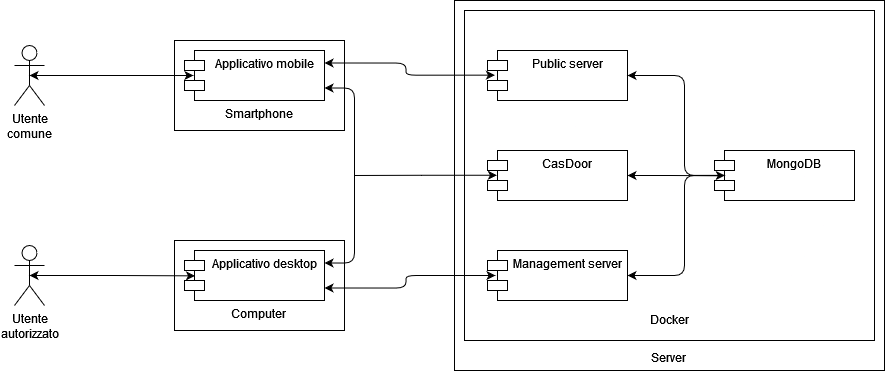
\includegraphics[width=1\textwidth]{Images/Component.png}
    \caption{Diagramma dell'architettura del sistema}
    \label{fig:architettura}
\end{figure}

\subsubsection{Configurazione di rete - integrazione componenti}
Tutti i \texttt{Docker Container}s sono in comunicazione tra di loro grazie a  \texttt{Docker Compose}, il quale crea una rete di default attraverso la quale tutti i container di un progetto possono comunicare tra di loro.
Questa rete è una rete "interna" e non accessibile dall'esterno. \texttt{Docker Compose} permette ovviamente di esporre esplicitamente alcuni container attraverso delle porte accessibili dall'esterno, che nel nostro caso sono:
\begin{itemize}
  \item Porta 27017 (localhost): Database MongoDB
	\item Porta 14124: Management Server
	\item Porta 7839: Public Server
	\item Porta 9987: Casdoor
\end{itemize}
Le applicazioni desktop e mobile sono configurate per accedere a queste porte. 
\\\\
\noindent
\textit{Nota: nel nostro deployment attivo, abbiamo effettuato ulteriori configurazioni di rete (e.g. per circumnavigare il NAT). Queste configurazioni sono trasparenti al resto del sistema e di conseguenza non le citeremo.}


\subsubsection{Requisiti di sistema}
Se si volesse effettuare un deployment locale del nostro sistema, allora la natura portabile dei containers Docker fa in modo che, virtualmente, qualsiasi sistema operativo sia capace di poter runnare il nostro progetto \texttt{Docker Compose}.\\
Parlando invece dei due applicativi, i requisiti minimi per la loro installazione e il loro funzionamento sono:
\begin{itemize}
    \item \textbf{Applicativo desktop}: Qualsiasi sistema operativo supportato da Flutter e Dart.
    \item \textbf{Applicativo mobile}: Sistema operativo Android 5.0 o superiore
\end{itemize}
È possibile utilizzarli anche come webapps, tuttavia non è stato previsto il loro deployment.

\clearpage

\subsubsection{Istruzioni per il deployment}
Si presuppone una conoscenza preliminare di Docker e Docker-Compose.
Le istruzioni per effettuare il deployment e il testing del nostro sistema (\texttt{backend}) sono presenti nel file \texttt{README.md} presente all'interno della nostra repository (nel branch \texttt{main}).


\subsubsection{Esecuzione applicativi mobile e desktop}
Provvederemo a fornire delle release già compilate dei due applicativi, in modo che non ci sia bisogno di compilarli da zero.\\
Gli applicativi mobile e desktop sono stati creati utilizzando Dart e il framework Flutter, per cui se si vuole effettuare il \texttt{build} degli applicativi è necessario avere un ambiente con tali elementi installati e configurati.
\\
Le istruzioni per compilare o installare gli applicativi mobile o desktop sono anch'essi all'interno del \texttt{README.md} presente all'interno del branch \texttt{main} della nostra repository. 

\subsubsection{Strumenti di monitoraggio}
Per monitorare il sistema e verificare che tutti i componenti siano in esecuzione e funzionanti è utilizzato Docker stesso, che permette di visualizzare lo stato dei container e delle risorse utilizzate.\\
Su un sistema con interfaccia grafica è possibile utilizzare Docker Desktop, mentre su un sistema senza interfaccia grafica è possibile utilizzare Docker CLI.
\begin{itemize}
    \item \textbf{Docker Desktop}
\end{itemize}
Docker Desktop è un'applicazione per desktop che permette di monitorare e gestire i container Docker in modo semplice e intuitivo.
\begin{itemize}
    \item \textbf{Docker CLI}
\end{itemize}
Docker CLI è un'interfaccia a riga di comando che permette di gestire i container Docker da terminale. Risulta meno intuitivo e più complesso rispetto a Docker Desktop, ma permette di ottenere le stesse funzionalità.\\
In questo caso d'uso, per monitorare i container in esecuzione, è utilizzato il comando \texttt{docker ps} che permette di visualizzare tutti i container in esecuzione e le informazioni principali su di essi.

\subsection{Stack tecnologico usato}
Per lo sviluppo del progetto abbiamo deciso, dopo approvazione della nostra proposta da parte dei docenti, di discostarci leggermente da quanto il corso prevedeva di utilizzare.\\
La descrizione che segue presenta su quali tecnologie sono ricadute le nostre scelte.

\subsubsection{Backend}
\textbf{Linguaggio di Programmazione: Rust}\\
Abbiamo scelto di usare Rust a causa del suo sistema di gestione della memory-safe e per le sue prestazioni elevate, nonchè per essere un linguaggio type-safe che induce gli utilizzatori a scrivere codice corretto e pulito. Consente inoltre di scrivere codice concorrenziale senza il rischio di data races, grazie al suo sistema di proprietà e borrowing.\\
Le librerie e i framework principali, che abbiamo utilizzato per creare il `management\_server` e il  `public\_server`, sono:
\begin{itemize}
    \item \textbf{Actix-web}: Actix-web è un framework asincrono per Rust utilizzato per costruire web servers; fornisce un'interfaccia semplice ed efficiente per la gestione delle richieste HTTP. Actix-web è nota per le sue prestazioni elevate e la capacità di gestire un gran numero di connessioni simultanee.
    \item \textbf{actix-web-httpauth}: Questa libreria viene utilizzata per l'autenticazione HTTP tramite Bearer tokens, permettendo di proteggere le API con token JWT.
    \item \textbf{jsonwebtoken}: Utilizzata per la gestione e la decodifica dei JSON Web Tokens (JWT), necessari per l'autenticazione e l'autorizzazione degli utenti.
    \item \textbf{\href{https://www.mongodb.com/docs/drivers/rust/current/}{mongodb}}: La connessione e le operazioni sul database sono gestite attraverso un il driver per Rust di MongoDB, permettendo l'interazione con il database MongoDB per la memorizzazione e il recupero dei dati.
\end{itemize}
Inoltre è stato sviluppato un modulo personalizzato per la gestione dell'autenticazione. Il modulo gestisce la decodifica e la verifica dei token JWT, utilizzando l'algoritmo RS256 per garantire la sicurezza dei token.\\
Per semplicità non è stato tuttavia impiegato TLS, il che rende vulnerabile il sistema.\\

\noindent
Si ricorda che la scelta di utilizzare un autenticatore esterno è stata ritenuta appropriata visto il contesto del progetto (Comune di Trento) nel quale si suppone siano già presenti sistemi di autenticazione.
La scelta di OpenID Connect potrebbe tuttavia essere limitante, visto il probabile utilizzo di SPID, basato su SAML.\\

\noindent
Per quanto riguarda la test-suite, è stata scritta utilizzando il framework di testing nativo di Rust \texttt{cargo test}.\\
I test sono stati scritti per verificare il corretto funzionamento delle API, controllando che le risposte siano corrette e che le richieste siano gestite correttamente.\\
E' stato sviluppato uno script di test per eseguire automaticamente tutti i test e verificare che tutte le funzionalità siano implementate correttamente attraverso un responso grafico e testuale dei risultati ottenuti.

\subsubsection{Frontend}
\textbf{Linguaggio di Programmazione: Dart}\\
Siccome era nostra intenzione quella di sviluppare due applicativi per tutte le interazioni possibili a sistema, la scelta del framework per lo sviluppo degli applicativi mobile e desktop sono ricaduti su Flutter, con conseguente utilizzo del linguaggio di programmazione Dart.\\
 Dart è un linguaggio sviluppato da Google, ottimizzato per lo sviluppo di applicazioni client su qualsiasi piattaforma. È particolarmente adatto per creare interfacce utente ricche e reattive.\\
Per lo sviluppo dello stile degli applicativi, sono state adoperate due librerie di stile differenti. Per quanto riguarda l'applicativo mobile è stata utilizzata la libreria \textbf{Material Design}, sviluppata da Google e caratteristica di Android, mentre per l'applicativo desktop è stata utilizzata la libreria \textbf{Fluent Design}, sviluppata da Microsoft e caratteristica dello stile del sistema Windows 11.\\
Come librerie aggiuntive abbiamo usato:
\begin{itemize}
    \item \textbf{flutter\_riverpod}: Utilizzato per la gestione dello stato nell'applicazione. Riverpod è un fornitore di gestione dello stato robusto e reattivo, che offre vantaggi come la sicurezza del tipo e il supporto per la dipendenza tra i provider.
    \item \textbf{CasdoorAuthenticationProvider}: Implementa un provider di autenticazione utilizzando Casdoor, un sistema di gestione delle identità e degli accessi. Il provider viene configurato con un segreto del client e un URL del server. \\
    Questa libreria ci permette di effettuare l'autenticazione degli utenti attraverso un portale fornito da Casdoor. 
    \item \textbf{JwtAuthenticator}: Utilizzato per autenticare gli utenti tramite JWT (JSON Web Tokens). Questo garantisce che le richieste API siano autorizzate e sicure.
\end{itemize}

\clearpage

\subsection{Conclusioni}

Possiamo quindi affermare che per il progetto BeeLive sono stati raggiunti con successo tutti gli obiettivi stabiliti per questo sprint:\\
Implementando le funzionalità di gestione degli eventi, si permette agli utenti autorizzati di creare, modificare ed eliminare eventi tramite l'applicazione desktop.\\
Gli utenti comuni, utilizzando l'applicazione mobile, possono visualizzare tutti i dettagli degli eventi, inclusi i sottoeventi.\\
L'architettura del sistema include il server pubblico (public\_server), il server di gestione (management\_server), il database MongoDB, il server di autenticazione Casdoor (Auth/Autn server), il servizio di routing OpenRouteService, l'applicazione desktop e l'applicazione mobile.\\

\noindent Nonostante il successo nel raggiungimento degli obiettivi del prodotto, l'applicazione del framework SCRUM ha per noi presentato alcune difficoltà, principalmente dovute alla necessità di focalizzarsi sull'implementazione tecnica.\\
La mancanza di test approfonditi sviluppati durante il primo sprint ha fatto emergere problematiche impreviste durante lo sviluppo, richiedendo modifiche che hanno coinvolto diverse user story contemporaneamente. Inoltre, l'interdipendenza tra le varie componenti del sistema ha reso complesso lavorare su singole user story in maniera isolata.\\
Queste sfide hanno portato il product backlog a trasformarsi in una lista di attività con priorità, orientata più sul prodotto che sull'utente finale.\\

\noindent Tuttavia, la stretta collaborazione tra noi membri del team, facilitata dalla comunicazione costante tramite Telegram e da incontri in presenza, ha permesso di superare queste difficoltà.\\
Come team, abbiamo tutti tratto vantaggio da un continuo scambio di conoscenze, specialmente per quanto riguarda gli aspetti tecnici del progetto, come l'uso di Dart, Rust e webtoken.\\

\noindent Guardando ai prossimi sprint, riteniamo che si potrebbe migliorare l'organizzazione SCRUM, formalizzando gli incontri del team per documentare i progressi e garantire che tutti i componenti del team siano allineati.\\
Inoltre, con le funzionalità principali del prodotto ormai completate, il team potrebbe aderire più rigorosamente alla metodologia, sfruttandone a pieno i suoi benefici.\\

\noindent Ad ogni modo è anche doveroso citare il fatto che si è notata una differenza netta tra il primo e questo secondo sprint. In questo ultimo periodo, a differenza di quello precedente, si è vista una maggiore collaborazione tra i membri del team, una maggiore comunicazione e una maggiore condivisione delle conoscenze.\\
Tutti questi aspetti, nel primo sprint, erano molto più altalenanti, in quanto non avendo mai avuto esperienze di lavoro in team sfruttando questo tipo di metotodologia, si è faticato molto di più a trovare un equilibrio.\\
Tutto era anche complicato dal fatto che nel primo sprint non c'erano basi o componenti già definite su cui iniziare a lavorare direttamente, quindi ogni componente del team si è focalizzato su una parte del progetto senza favorire la visione d'insieme.\\
Questo secondo sprint, invece, è stato molto più fluido e ha permesso di lavorare in modo più efficiente e produttivo tra tutti noi membri del team, dando molta più enfasi alla collaborazione piuttosto che al compimento del singolo task.\\
\end{document}
